\documentclass[12pt,a4paper]{article}

\usepackage[utf8]{inputenc}
\usepackage[T1]{fontenc}
\usepackage{geometry}
\geometry{margin=2.5cm}
\usepackage{setspace}
\onehalfspacing
\usepackage{graphicx}
\usepackage{booktabs}
\usepackage{tabularx}
\usepackage{amsmath}
\usepackage{amssymb}
\usepackage{hyperref}
\hypersetup{colorlinks=true, linkcolor=blue, citecolor=blue, urlcolor=blue}
\usepackage{parskip}
\usepackage{tikz}
\usetikzlibrary{arrows.meta, positioning, shapes.geometric, fit, backgrounds, calc}
\usepackage{xcolor}
\definecolor{cprsblue}{HTML}{2C7FB8}
\definecolor{cprsgreen}{HTML}{31A354}
\definecolor{cprsgrey}{HTML}{6E6E6E}

\newcommand{\ndcg}{nDCG}
\newcommand{\RQ}[1]{\textbf{RQ#1}}

\title{\textbf{CPRS: A Cross-Platform Competitive Programming Recommendation System} \\[1em]
\large CM3070 Computer Science Final Project --- Final Report \\[0.5em]
\large Template 1.1: Data-Driven Personalised Educational Content Recommendation}
\author{}
\date{}

\begin{document}

%---------------------------------------------------------------- title page
\begin{titlepage}
\centering
\vspace*{2.5cm}
{\Huge\bfseries CPRS: A Cross-Platform\\[0.3em] Competitive Programming\\[0.3em]
Recommendation System\par}
\vspace{2cm}
{\Large CM3070 Computer Science Final Project\par}
\vspace{0.4em}
{\Large\itshape Final Report\par}
\vspace{1.2em}
{\large Template 1.1: Data-Driven Personalised\\Educational Content Recommendation\par}
\vfill
{\large \textbf{Author:}\quad\rule{5cm}{0.4pt}\par}
\vspace{0.4em}
{\large \textbf{Student ID:}\quad\rule{5cm}{0.4pt}\par}
\vspace{1.5em}
{\large \today\par}
\end{titlepage}

%---------------------------------------------------------------- abstract
\pagenumbering{roman}
\begin{abstract}
\noindent Competitive-programming platforms host millions of problems but give
users little personalised guidance on what to solve next, and each platform is an
isolated silo with its own difficulty scale and tag taxonomy. This project builds
CPRS, a cross-platform recommender spanning Codeforces, AtCoder, CodeChef and
LeetCode. We curate a unified dataset of 45{,}903 problems with normalised difficulty
and a shared taxonomy of 43 canonical topics, recover AtCoder's missing topic tags
with an NLP transfer tagger, and assemble a real user$\times$problem interaction dataset
(2{,}459 users, 532{,}059 solves) by sampling the Codeforces API. On a held-out
temporal split we compare six recommenders under five ranking metrics with paired
significance testing. Collaborative filtering dominates (\ndcg{}@10 $=0.096$, versus
$0.037$ for a popularity baseline; $p<10^{-42}$), while a content baseline is shown to
be mis-aligned with next-solve prediction. We then interrogate the project's central
premise --- that \emph{cross-platform data} improves recommendation. That premise
survives only in a specific, and initially surprising, form. Collaborative transfer
across platforms fails: the problem sets are disjoint and, empirically, multi-platform
users are experienced on every platform, so the cold population the idea targets
barely exists. Yet \emph{skill} transfers strongly --- on the unified difficulty scale
a user's Codeforces and AtCoder skill correlate at $r=0.77$ --- and an online
cross-platform skill estimator exploits this to predict a brand-new user's ability
$35$--$40\%$ more accurately than a population prior, correcting itself as evidence
accrues. The contribution is thus a curated cross-platform resource and NLP tagger,
together with a rigorous, evidence-driven account of \emph{when} collaborative,
content and cross-platform signals help --- including several counter-intuitive but
well-explained negative results that sharpen the boundary of a commonly assumed
benefit.
\end{abstract}

\newpage
\setcounter{tocdepth}{2}
\tableofcontents
\newpage
\pagenumbering{arabic}

%======================================================================
\section[Introduction \textnormal{\small(1,000 words)}]{Introduction}
\label{sec:intro}
%======================================================================

\subsection{Motivation and Context}
Competitive programming has grown into a global educational practice. Platforms such
as Codeforces, AtCoder, CodeChef and LeetCode collectively host millions of algorithmic
problems
and serve tens of millions of users~\cite{wasik2018}, functioning both as training
grounds for algorithmic reasoning and as \emph{de-facto} assessment instruments in
technical hiring, where developers report that preparation centres on exactly this kind
of timed algorithmic problem~\cite{behroozi2019}. Their very scale, however, creates a discovery
problem: a learner must repeatedly decide \emph{which problem to attempt next} from a
space of thousands, usually by trial and error or informal peer advice rather than
systematic, personalised guidance. Because timely, well-targeted feedback is central
to skill acquisition~\cite{boud2013}, this is a genuine educational deficiency, not a
mere convenience gap; yet platforms surface only coarse aggregate statistics (a rating,
a solve count) and no actionable problem-level direction.

The scale of that decision is worth making concrete, because it is easy to underestimate.
In the unified catalogue assembled for this project (Section~\ref{sec:design-data}),
$1{,}685$ problems sit within $\pm0.05$ of the median learner's skill on the normalised
difficulty scale --- that is, roughly seventeen hundred problems are all plausibly
``the right level'' at any given moment, before topic, style or novelty are considered at
all. A learner cannot inspect that set, so in practice they sample from a small, biased
corner of it: in our interaction data the most-solved tenth of problems absorbs
$51\%$ of all solve events, while the median problem is solved by just $23$ of $2{,}459$
users. The consequence is not merely inefficiency but systematic distortion --- practice
concentrates on whatever is visible rather than on whatever would most improve the
learner. This is the discovery problem the project sets out to address, and it is
precisely the shape of problem that personalised ranking exists to solve.

The difficulty is compounded by \emph{fragmentation}. Each platform operates as an
island with its own difficulty scale, tag taxonomy and user base. A learner practising
on Codeforces receives no guidance about complementary AtCoder or LeetCode problems
that would target the same weakness, and the rich behavioural trace a user generates on
one platform is invisible to the others. Existing aids --- platform-curated lists,
community ``ladders'', forum advice --- are neither personalised nor cross-platform.
Bridging these islands is the specific opportunity CPRS pursues.

\subsection{Problem Statement}
This project addresses the question: \emph{can data-science techniques build a
personalised competitive-programming recommender that operates across platforms, and
does cross-platform data measurably improve recommendation quality?} The second clause
is not rhetorical. Cross-platform value is widely \emph{assumed} by systems that
aggregate profiles, but --- as far as we are aware --- never \emph{measured}. A central
aim of this work is to test it directly, and the answer proves more nuanced than the
premise.

\subsection{Aims and Objectives}
\label{sec:objectives}
The overall aim is a working, evaluated cross-platform recommender that is both a
useful tool and a vehicle for answering the research questions below. Concretely, the
measurable objectives are:
\begin{enumerate}
    \item[\textbf{O1}] Curate a unified, normalised cross-platform problem dataset
    (comparable difficulty, shared tag taxonomy, stable identifiers).
    \item[\textbf{O2}] Recover AtCoder's missing topic tags with an NLP method,
    evaluated by cross-validation.
    \item[\textbf{O3}] Assemble a real user$\times$problem interaction dataset and a
    principled (temporal) train/test protocol.
    \item[\textbf{O4}] Implement and compare content-based, collaborative and hybrid
    recommenders under standard ranking metrics with statistical significance.
    \item[\textbf{O5}] Characterise cold-start behaviour and derive an evidence-based
    cold-start policy.
    \item[\textbf{O6}] Determine empirically whether, and how, cross-platform history
    improves recommendation.
    \item[\textbf{O7}] Deliver a working web application that builds live
    multi-platform profiles and serves recommendations.
\end{enumerate}

\subsection{Research Questions}
The evaluation (Sections~\ref{sec:eval}--\ref{sec:results}) is organised around four
questions:
\begin{itemize}
    \item[\RQ{1}] Which recommendation paradigm best predicts what a user solves next
    --- content-based, collaborative filtering, or a hybrid?
    \item[\RQ{2}] How do recommenders behave under \emph{cold start}, and what is the
    correct cold-start policy?
    \item[\RQ{3}] Does merging a user's cross-platform history improve
    \emph{collaborative} recommendation on a target platform?
    \item[\RQ{4}] Is skill itself transferable across platforms on a unified difficulty
    scale, and can it be exploited for cold start?
\end{itemize}

\subsection{Contributions}
\label{sec:contributions}
\begin{enumerate}
    \item \textbf{A curated cross-platform dataset} of 45{,}903 problems over four
    judges with min--max-normalised difficulty and a 43-topic unified taxonomy, plus an
    interaction dataset of 2{,}459 users and 532{,}059 solves, time-split for offline
    evaluation (Sections~\ref{sec:design-data}, \ref{sec:impl-data}).
    \item \textbf{An NLP cross-platform transfer tagger} recovering absent topic tags on
    two further platforms from Codeforces statements, with a calibrated cross-validated
    evaluation and a two-tier finding about which tags are text-learnable
    (Section~\ref{sec:tagger}).
    \item \textbf{A rigorous comparative evaluation} of six recommenders across five
    ranking metrics, with activity slicing, a cold-start fold-in simulation, paired
    Wilcoxon tests and bootstrap confidence intervals (Section~\ref{sec:results}).
    \item \textbf{The cross-platform value study} (\RQ{3}--\RQ{4}): collaborative
    transfer fails but skill transfer succeeds ($r=0.77$), and an \textbf{online
    cross-platform skill estimator} improves cold-start skill estimation by
    $35$--$40\%$ (Sections~\ref{sec:design-skill}, \ref{sec:results-xplat}).
    \item \textbf{A working web application} that builds live multi-platform user
    profiles and serves cross-platform recommendations (Section~\ref{sec:impl-web}).
\end{enumerate}

\subsection{An Evidence-Driven Journey}
\label{sec:journey}
This project did not unfold as planned, and the divergence is the source of its best
findings. We set out expecting a
\emph{hybrid} recommender to be the centrepiece and cross-platform aggregation to be an
obvious win. The data refused both expectations. The hybrid did not beat collaborative
filtering; cross-platform \emph{collaborative} transfer actively hurt; and the
population that cross-platform cold-start was meant to rescue turned out to barely
exist. Rather than discard the premise, we followed the evidence to a sharper question
--- is \emph{skill}, as opposed to co-occurrence, transferable? --- and found that it
is, strongly. The report is written to make this reasoning visible: each major result
is presented as a hypothesis tested, sometimes refuted, and refined --- more honest, and
more instructive, than a tidy narrative in which everything worked.

\subsection{Report Structure}
Section~\ref{sec:lit} reviews the literature and states the gap. Section~\ref{sec:design}
gives requirements and design; Section~\ref{sec:impl} the implementation.
Section~\ref{sec:tagger} presents the NLP tagger. Section~\ref{sec:eval} defines the
evaluation methodology and Section~\ref{sec:results} reports the results, threaded as an
inquiry. Section~\ref{sec:discussion} discusses them against the objectives,
Section~\ref{sec:ethics} covers professional and ethical considerations, and
Section~\ref{sec:conclusion} concludes. Appendices give full metric tables,
hyperparameters, the taxonomy and reproduction instructions.

%======================================================================
\section[Literature Review \textnormal{\small(1,378 words)}]{Literature Review}
\label{sec:lit}
%======================================================================

\subsection{Recommender Systems: Foundations}
Recommender systems are conventionally grouped into three families~\cite{ricci2015}.
\emph{Content-based} methods represent items by features and recommend those similar to
a user's profile~\cite{lops2011}; they handle new items gracefully but tend to
over-specialise and cannot discover interests outside a user's established profile.
\emph{Collaborative filtering} (CF) instead exploits patterns of co-occurrence across
users' behaviour, needing no item features. \emph{Hybrid} systems combine paradigms to
offset each other's weaknesses~\cite{burke2002}, and in the recommender literature are
routinely the strongest performers --- an expectation this project set out to confirm
and, instructively, did not (Section~\ref{sec:results}).

\subsection{Matrix Factorisation and Implicit Feedback}
Latent-factor models via matrix factorisation are the dominant CF
approach~\cite{koren2009}: users and items are embedded in a shared low-dimensional
space and affinity is their inner product. Most competitive-programming signal is
\emph{implicit} --- we observe that a user \emph{solved} a problem, but not a graded
preference, and non-solves are ambiguous (unseen vs.\ failed vs.\ disliked). Hu, Koren
and Volinsky~\cite{hu2008} address this with a confidence-weighted alternating least
squares (ALS) formulation that treats observed interactions as positive preference with
a confidence that grows with interaction strength; it is the model we adopt.
Bayesian Personalised Ranking~\cite{rendle2009} offers a pairwise-ranking alternative
optimised directly for ordering. A persistent limitation of all CF is
\emph{cold start}~\cite{schein2002}: a user or item with little history cannot be
placed in the latent space --- the precise failure our cross-platform skill model
targets.

\subsection{Cross-Domain and Transfer Recommendation}
Directly relevant to this project is \emph{cross-domain} recommendation, which seeks to
transfer knowledge from a source domain (here, one platform) to improve a target
domain~\cite{cantador2015}. Cantador et al.\ organise the field by what the domains have
in common, and the distinction turns out to be decisive for our results. Transfer may
proceed over shared \emph{items} (the same films rated on two sites), shared
\emph{users} (the same person active in two domains), or a shared \emph{latent space}
inferred by tying the two factorisations together~\cite{pan2010}. Pan et al.\ show that
when neither users nor items overlap, transfer must instead move a \emph{rating pattern}
--- a compressed regularity abstracted away from the specific entities --- and that the
success of the transfer depends entirely on whether such a shared regularity genuinely
exists rather than on the machinery used to move it.

The competitive-programming setting is an unusually clean instance of the user-overlap
case, and this is what makes it a good testbed. Platforms share \emph{users}, because
competitive programmers commonly reuse a handle across judges, but they share almost no
\emph{items}: a Codeforces problem and an AtCoder problem are distinct artefacts, and the
catalogues do not intersect at all. The literature is explicit that this is the harder
configuration. With no shared items there is no anchor forcing the two domains' latent
spaces into a common frame, so a naive joint factorisation is free to place each domain's
factors in whatever subspace best explains its own observations, and the resulting
geometry need not be comparable across domains~\cite{cantador2015,pan2010}. Our Design~A
and~B experiments (Section~\ref{sec:results-xplat}) reproduce exactly this failure, and
we regard that as a confirmation of the theory rather than a defect of the
implementation.

What the theory also suggests, read carefully, is the way out. If transfer requires a
shared regularity that is not tied to particular items, then the productive question is
which construct in this domain has that property. Item co-occurrence plainly does not:
it is defined over a catalogue, and the catalogues are disjoint. \emph{Ability}, by
contrast, is a property of the learner that the knowledge-tracing literature below treats
as existing independently of any particular item set --- which makes it precisely the kind
of domain-independent regularity Pan et al.\ describe. That observation is what redirects
this project from collaborative transfer to skill transfer, and
Section~\ref{sec:results-xplat} shows it is empirically correct.

\subsection{Sequence- and Session-Aware Recommendation}
Because a learner's next choice depends on recent activity, session-based recommenders
that model interaction order --- e.g.\ recurrent approaches such as
GRU4Rec~\cite{hidasi2016} --- are conceptually attractive here. They also raise the bar
for evaluation, motivating a \emph{temporal} rather than random train/test split so
that predicting the future from the past is genuinely tested~\cite{cremonesi2010}. We
adopt temporal evaluation throughout; a full sequence model was scoped as future work
(Section~\ref{sec:conclusion}) to keep the critical path on the cross-platform question.

\subsection{Knowledge Tracing and Ability Modelling}
Modelling a learner's evolving ability is the subject of knowledge tracing. Bayesian
Knowledge Tracing~\cite{corbett1994} and Deep Knowledge Tracing~\cite{piech2015} track
per-skill mastery over time. Item Response Theory~\cite{pelanek2017} and the Elo rating
system~\cite{elo1978} model the probability of a correct response as a logistic function
of the gap between learner ability and item difficulty --- the same functional form we
use for solvability (Section~\ref{sec:design-skill}). Vygotsky's ``zone of proximal
development''~\cite{vygotsky1978} provides the pedagogical rationale for recommending
problems slightly above current ability, which our difficulty-matching scorer
operationalises. Crucially, ability in these frameworks is a property of the
\emph{learner}, not of any single item set --- foreshadowing why skill, unlike
item co-occurrence, transfers across platforms.

\subsection{Recommendation in Programming Education}
Recommendation for online judges is a small but established literature, and two studies
are especially close to this project. Yera Toledo et al.~\cite{yera2018} recommend
problems on a programming online judge by modelling problem difficulty and learner
ability as fuzzy quantities, and report that difficulty-aware recommendation beats
difficulty-agnostic collaborative filtering. Their result is an early signal that
\emph{ability} is the load-bearing construct in this domain --- a conclusion our own
evidence reaches from an entirely different direction (Section~\ref{sec:results}), and
which we extend by showing that ability is also the quantity that survives a change of
platform. Zhao et al.~\cite{zhao2018} jointly infer problem \emph{topics} and
\emph{difficulty levels} from online-judge submission logs with a unified probabilistic
model, establishing that metadata a platform never published can be recovered from the
data it does expose. Our NLP tagger (Section~\ref{sec:tagger}) attacks the same
metadata-scarcity problem from the complementary direction --- problem statements rather
than behaviour logs --- and our per-tag analysis contributes a finding their aggregate
figures cannot show: \emph{which} labels are recoverable from text at all, and why a
whole class of them is not.

Two limitations run through this work, and together they define our opening. First, it
is uniformly \emph{single-platform}. Each system is trained and evaluated on one judge,
so neither the portability of its constructs nor the value of aggregating evidence
across judges is ever put to the test; cross-platform benefit is left as an assumption
that no one has had the data to check. Second, evaluation tends to be narrow --- one
dataset, one or two accuracy metrics, and frequently no strong non-personalised
reference point --- which is precisely the practice that Cremonesi et
al.~\cite{cremonesi2010} and Dacrema et al.~\cite{dacrema2019} identify as a source of
overstated progress in recommender research generally. Outside academia the picture is
weaker still: the tools competitive programmers actually use day to day are community
projects (topic ladders, weakness finders, rating predictors) that are heuristic,
undocumented and, as far as we can establish, never evaluated against a baseline at all.
The result is a domain in which practice is already cross-platform --- learners routinely
hold accounts on several judges --- while neither the literature nor the tooling has
measured whether crossing platforms actually helps. That untested assumption is the gap
this project targets, and Section~\ref{sec:results-xplat} shows that testing it
overturns the obvious answer.

\subsection{Evaluation Methodology and its Pitfalls}
Offline top-$N$ evaluation is standard but subtle. Ranking quality is measured with hit
rate, precision/recall@$K$, mean reciprocal rank and normalised discounted cumulative
gain (\ndcg{})~\cite{jarvelin2002}. Cremonesi et al.~\cite{cremonesi2010} show that such
metrics must be read against strong baselines --- popularity in particular is
deceptively hard to beat --- and that a temporal split better reflects deployment than a
random one. Because per-user metric distributions are non-normal and zero-inflated,
model differences should be tested with a paired non-parametric test such as the
Wilcoxon signed-rank test~\cite{wilcoxon1945}, reported with effect sizes and confidence
intervals rather than point estimates alone~\cite{dacrema2019}. We follow these
recommendations throughout, and they materially shape our conclusions.

\subsection{Gap Analysis and Contribution Mapping}
The literature supplies mature single-platform techniques and clear evaluation practice,
but leaves the cross-platform question open and, where cross-domain transfer is studied,
warns that user-overlap transfer is fragile. Table~\ref{tab:gap} maps each gap to the
contribution that addresses it.

\begin{table}[h]
\centering
\caption{Gaps identified in the literature and the contributions that address them.}
\label{tab:gap}
\small
\begin{tabularx}{\textwidth}{@{}p{5.4cm}X@{}}
\toprule
\textbf{Gap in prior work} & \textbf{CPRS contribution} \\
\midrule
No dataset unifies behaviour or problems across CF/AtCoder/CodeChef/LeetCode & Curated
unified catalogue (45{,}903 problems) + real interaction dataset (\S\ref{sec:design-data},
\S\ref{sec:impl-data}) \\
AtCoder problems lack topic tags, preventing topic-based analysis & NLP transfer tagger
from CF statements, cross-validated (\S\ref{sec:tagger}) \\
Community tools are rarely evaluated with ranking metrics or baselines & Six-model
comparison, five metrics, significance testing (\S\ref{sec:results}) \\
Cross-platform value is assumed, never measured & Direct study: collaborative transfer
fails; skill transfer succeeds ($r=0.77$) (\S\ref{sec:results-xplat}) \\
Cross-domain transfer over shared users is known to be fragile, but untested here &
Two mechanisms tested and refuted; a shared-ability alternative validated
(\S\ref{sec:results-xplat}) \\
Cold start asserted rather than characterised & Fold-in simulation + an online
cross-platform skill estimator (\S\ref{sec:design-skill}) \\
\bottomrule
\end{tabularx}
\end{table}

%======================================================================
\section[Requirements and Design \textnormal{\small(1,522 words)}]{Requirements and Design}
\label{sec:design}
%======================================================================

\subsection{Requirements}
\label{sec:requirements}
The target users are competitive programmers across the ability range --- beginners
choosing early problems, intermediates navigating the largest and most heterogeneous
problem space, and advanced users seeking targeted practice --- as well as candidates
preparing for technical interviews. From this the following requirements follow.

\paragraph{Functional.} (F1) ingest problems from Codeforces, AtCoder, CodeChef and
LeetCode into a unified schema; (F2) normalise difficulty to a common scale and tags to a common
taxonomy; (F3) infer missing AtCoder tags; (F4) build a user skill profile from
submission history on any supported platform; (F5) generate a ranked, personalised
problem list drawing from all platforms; (F6) present recommendations with difficulty,
topic and a link to the origin judge; (F7) refresh a profile as the user solves more.

\paragraph{Non-functional.} (N1) recommendations computed offline in seconds over
$\sim$$10^4$ problems and $\sim$$10^3$ users; (N2) reproducible data pipeline with frozen
raw data; (N3) respectful use of third-party APIs (rate limiting, caching); (N4) safe
handling of user credentials; (N5) evaluability --- every claim supported by a metric
and, where comparative, a significance test.

\subsection{Platform Selection}
\label{sec:design-platforms}
Which judges to support is the first design decision, and it constrains every later
one: a platform that cannot be joined to the others contributes nothing but rows. The
requirements above imply three distinct things a candidate must supply, and they are not
equally easy to obtain. A judge must expose (i) an enumerable \emph{catalogue} of
problems, (ii) a per-problem \emph{difficulty} signal, without which F5's difficulty
matching cannot rank it, and (iii) a public per-user \emph{solve history}, without which
its users cannot enter the interaction matrix at all. Layer (iii) is the binding
constraint, because it is the only one a platform can withhold outright.

Table~\ref{tab:platforms} surveys the candidates against these three layers. The
right-hand column reports the fraction of our Codeforces cohort holding an account under
the same handle --- the mechanism by which a second platform is bridged to the first
(Section~\ref{sec:impl-cohort}) --- measured by probing a random sample of handles.

\begin{table}[h]
\centering
\caption{Platform survey. \emph{History} is public per-user solve data; \emph{overlap} is
the share of sampled Codeforces handles with an account of the same name. Adopted
platforms in bold.}
\label{tab:platforms}
\small
\begin{tabular}{llccccl}
\toprule
Platform & Access & Catalogue & Difficulty & Tags & Overlap & Outcome \\
\midrule
\textbf{Codeforces} & REST API  & 11{,}263 & rating   & yes  & ---   & adopted (anchor) \\
\textbf{AtCoder}    & community & 9{,}095  & modelled & no   & 15.5\% & adopted \\
\textbf{CodeChef}   & site JSON & 21{,}568 & partial  & weak & 20\%  & adopted \\
\textbf{LeetCode}   & GraphQL   & 3{,}977  & ordinal  & yes  & ---   & adopted (catalogue) \\
\midrule
DMOJ        & REST API    & 5{,}269 & points & yes & 2\% & rejected: no bridge \\
HackerRank  & internal    & tracks  & none   & yes & --- & rejected: no difficulty \\
Codewars    & REST API    & no list & kyu    & yes & --- & rejected: not contest problems \\
Kattis      & HTML only   & scraped & 1--10  & no  & --- & rejected: scrape-only \\
CSES        & HTML only   & 300     & none   & no  & --- & rejected: nothing to normalise \\
Aizu        & API removed & ---     & ---    & --- & --- & rejected: endpoint withdrawn \\
\bottomrule
\end{tabular}
\end{table}

The survey yields a conclusion sharper than the selection itself, and one that
generalises beyond this project: \emph{the cost of adding a platform is set by how it
exposes user histories, not by the quality of its API}. DMOJ has the cleanest interface
of anything surveyed --- a documented, versioned REST API serving public per-user
submissions without authentication --- and is nonetheless useless here, because only
$2\%$ of our cohort holds an account, leaving too thin a bridge to learn anything
across. CodeChef inverts every one of those properties: its official API has been
withdrawn, its histories must be walked a dozen rows of HTML at a time, and it throttles
aggressively enough to force exponential backoff --- yet it matches $20\%$ of the cohort,
a denser bridge than AtCoder's, and so earns its place. API quality is a cost; overlap is
the value, and the two are uncorrelated.

Three further asymmetries shaped what each adopted platform is used \emph{for}, rather
than whether to adopt it. Codeforces is the anchor because it alone couples a large
public catalogue to unrestricted submission histories, which is why the evaluation is
conducted Codeforces-side. LeetCode publishes only the most recent accepted submissions
per user, so it contributes a catalogue and a live profile but no evaluable history.
CodeChef, uniquely, reports \emph{every} verdict rather than only successes, so
attempted-but-unsolved problems are directly observable there --- the negative signal
whose absence bounds the models elsewhere (Section~\ref{sec:threats}).

\subsection{System Architecture}
CPRS is organised as a data pipeline feeding a set of recommendation models, exposed
through a web application (Figure~\ref{fig:arch}). Fetchers for the four platforms of
Section~\ref{sec:design-platforms} collect raw problem
catalogues and user submissions; an ETL stage normalises them into a unified schema; the
NLP tagger enriches AtCoder problems; and the recommendation models are evaluated
offline and served live.

\begin{figure}[h]
\centering
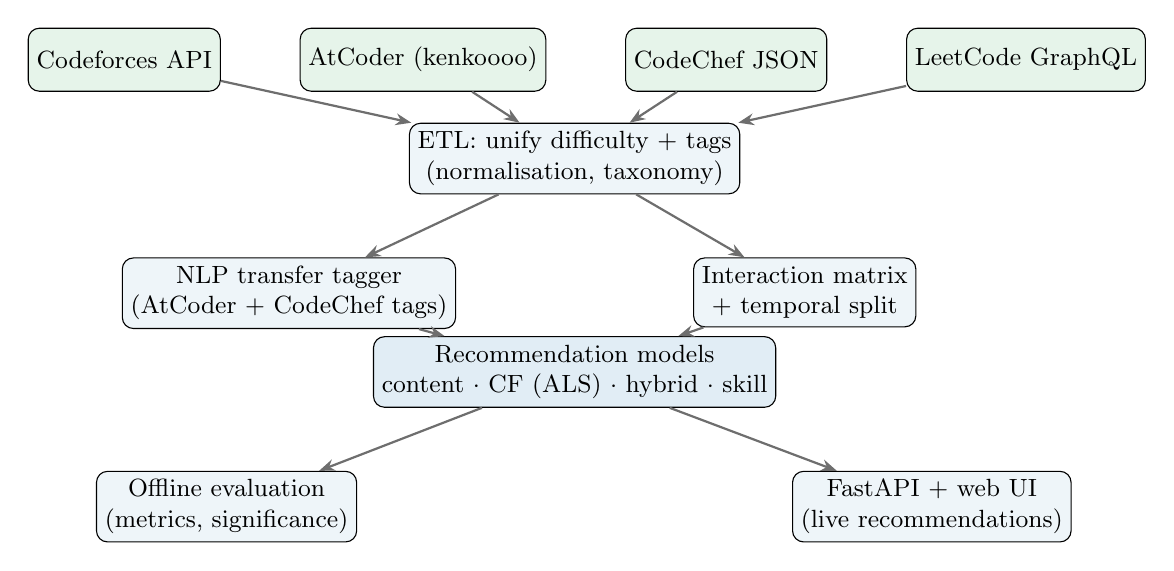
\begin{tikzpicture}[
    node distance=6mm and 10mm,
    box/.style={draw, rounded corners, align=center, minimum height=8mm,
                inner sep=3pt, font=\small, fill=cprsblue!8},
    src/.style={box, fill=cprsgreen!12},
    mdl/.style={box, fill=cprsblue!14},
    arr/.style={-{Stealth[length=2mm]}, cprsgrey, thick}]
  \node[src] (cf) {Codeforces API};
  \node[src, right=of cf] (ac) {AtCoder (kenkoooo)};
  \node[src, right=of ac] (cc) {CodeChef JSON};
  \node[src, right=of cc] (lc) {LeetCode GraphQL};
  \node[box, below=8mm of $(ac)!0.5!(cc)$] (etl) {ETL: unify difficulty + tags\\(normalisation, taxonomy)};
  \node[box, below left=8mm and -6mm of etl] (tag) {NLP transfer tagger\\(AtCoder + CodeChef tags)};
  \node[box, below right=8mm and -6mm of etl] (mat) {Interaction matrix\\+ temporal split};
  \node[mdl, below=18mm of etl] (models) {Recommendation models\\content $\cdot$ CF (ALS) $\cdot$ hybrid $\cdot$ skill};
  \node[box, below left=8mm and 2mm of models] (eval) {Offline evaluation\\(metrics, significance)};
  \node[box, below right=8mm and 2mm of models] (app) {FastAPI + web UI\\(live recommendations)};
  \draw[arr] (cf) -- (etl); \draw[arr] (ac) -- (etl);
  \draw[arr] (cc) -- (etl); \draw[arr] (lc) -- (etl);
  \draw[arr] (etl) -- (tag); \draw[arr] (etl) -- (mat);
  \draw[arr] (tag) -- (models); \draw[arr] (mat) -- (models);
  \draw[arr] (models) -- (eval); \draw[arr] (models) -- (app);
\end{tikzpicture}
\caption{CPRS system architecture: from platform APIs through unification and tagging to
models, offline evaluation and the served application.}
\label{fig:arch}
\end{figure}

\subsection{Unified Data Schema and Difficulty Normalisation}
\label{sec:design-data}
The four platforms express difficulty incompatibly: Codeforces uses an integer rating
(roughly 800--3500); AtCoder uses a community model-estimated real value that can be
negative~\cite{kenkoooo2024}; CodeChef publishes an Elo-like problem rating for only a
quarter of its catalogue; LeetCode uses three ordinal levels. We map all four onto a
common $[0,1]$ scale by min--max normalisation with platform-specific bounds
(Figure~\ref{fig:difficulty}):
\begin{align}
d_{\text{CF}}   &= \operatorname{clip}\!\Big(\tfrac{r-800}{3500-800},\,0,\,1\Big), &
d_{\text{AC}}   &= \operatorname{clip}\!\Big(\tfrac{b+500}{4000+500},\,0,\,1\Big), \\
d_{\text{CC}}   &= \operatorname{clip}\!\Big(\tfrac{r-200}{4000-200},\,0,\,1\Big), &
d_{\text{LC}}   &\in \{0.2,\,0.5,\,0.85\}.
\end{align}
\begin{figure}[h]
\centering
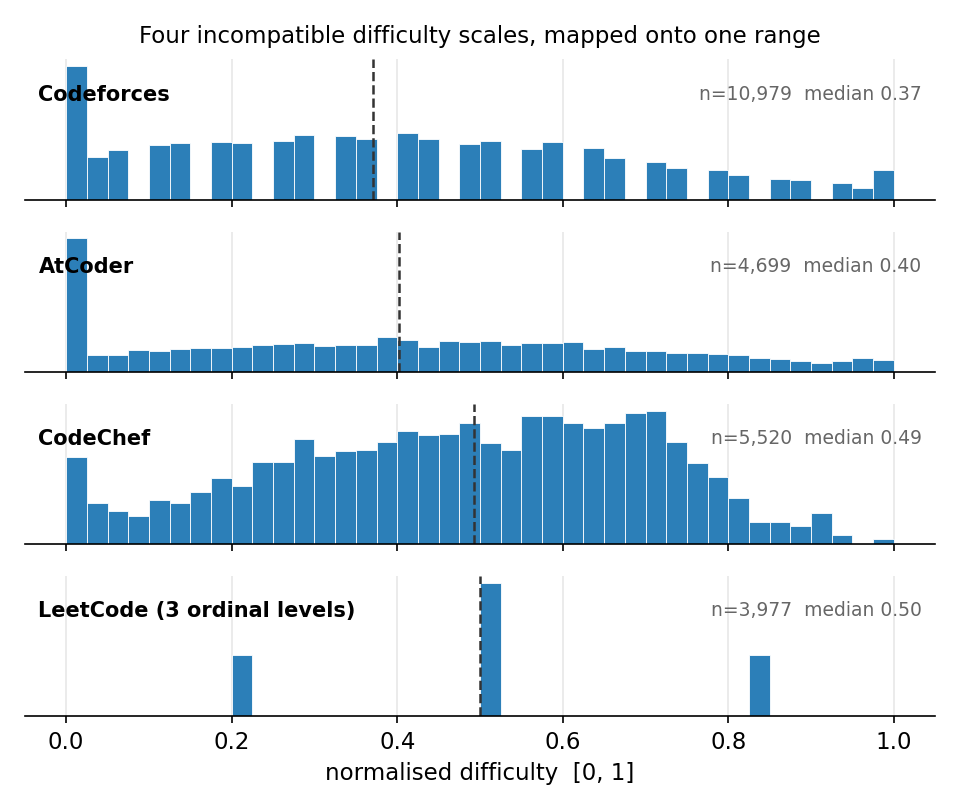
\includegraphics[width=0.82\textwidth]{figures/difficulty_by_platform.png}
\caption{Catalogue difficulty per platform on the unified scale. The mapping brings four
incompatible scales into one range but does not make them identical: medians run from
$0.37$ (Codeforces) to $0.50$ (LeetCode), so a cross-platform match is approximate rather
than exact. The spike at $0$ for Codeforces and AtCoder is the lower clip, and LeetCode
resolves to three spikes because it publishes only three ordinal levels. It is this
scale, not the distributions' shape, that the $r=0.77$ skill correlation of
Section~\ref{sec:results-xplat} validates.}
\label{fig:difficulty}
\end{figure}

Unlike the other three, CodeChef publishes no documented rating range, so its bounds are
set empirically from the catalogue: over the $5{,}520$ rated problems of $21{,}568$,
ratings span $19$--$4076$ with 1st and 99th percentiles at $193$ and $3660$, so
$[200, 4000]$ covers the mass while clipping a thin tail at each end. Unrated problems
are flagged by sentinel values rather than omitted, and are rejected rather than
silently normalised to zero.
Tags from all platforms are folded into a shared taxonomy of 43 canonical topics
(Appendix~\ref{app:taxonomy}), and every problem receives a stable identifier
(\texttt{cf:1234A}, \texttt{ac:abc123\_a}, \texttt{lc:42}). Two assumptions are explicit:
that difficulty distributions are roughly comparable across platforms after
normalisation, and that AtCoder's model-derived difficulty is a usable proxy. Rather than
take these on faith we test the first directly (Section~\ref{sec:results-xplat}), and it
is the empirical validation of this scale ($r=0.77$) that ultimately carries the
cross-platform contribution.

\subsection{Recommendation Models}
\label{sec:design-models}
All models share one interface --- given a user, produce a real-valued score over every
candidate problem --- so they can be ranked, masked and blended uniformly.

\paragraph{Content-based.} A problem $p$ with unified tags $T_p$, difficulty $d_p$ and
solve-count popularity is scored against a user profile built from their solved
problems. Two deliberately opposed variants are studied. The \emph{pedagogical} scorer
combines a topic-gap term (favouring \emph{unseen}/weak topics), a difficulty-fit
Gaussian centred \emph{above} the user's level (stretch), and popularity:
\begin{equation}
s^{\text{ped}}_p = 0.4\,g_u(T_p) + 0.4\,\exp\!\Big(\!-\tfrac{(d_p-(\theta_u+\sigma_s))^2}{2\sigma^2}\Big) + 0.1\,\hat{\rho}_p ,
\end{equation}
where $g_u$ is the mean inverse-mastery of $p$'s tags, $\theta_u$ the user's level and
$\hat\rho_p$ log-scaled popularity. The \emph{difficulty-match} scorer
(\texttt{diffmatch}) instead favours \emph{familiar} topics at \emph{at-level}
difficulty:
\begin{equation}
s^{\text{match}}_p = 0.5\,f_u(T_p) + 0.5\,\exp\!\Big(\!-\tfrac{(d_p-\theta_u)^2}{2\sigma^2}\Big) + 0.05\,\hat{\rho}_p ,
\end{equation}
with $f_u$ the mean \emph{familiarity} (solve count) of $p$'s tags. The contrast --- push
toward the unfamiliar and hard, versus stay near the familiar and comfortable --- is a
design probe whose effect the evaluation measures directly.

\paragraph{Collaborative filtering.} We factorise the binary user$\times$problem ``solved''
matrix $R$ with implicit-feedback ALS~\cite{hu2008}, minimising
$\sum_{u,p} c_{up}\big(\mathbb{1}[R_{up}{>}0]-x_u^\top y_p\big)^2 + \lambda(\lVert x_u\rVert^2+\lVert y_p\rVert^2)$
with confidence $c_{up}=1+\alpha R_{up}$. A user's score for a problem is $x_u^\top y_p$.

\paragraph{Hybrid and cold-start mechanism.} CF and a ``cold'' ingredient (content or
popularity) are min--max normalised per user and blended by interaction density:
\begin{equation}
s^{\text{hyb}}_p = \alpha(n_u)\,\widetilde{s}^{\,\text{cf}}_p + \big(1-\alpha(n_u)\big)\,\widetilde{s}^{\,\text{cold}}_p ,
\qquad \alpha(n_u)=\frac{n_u}{n_u+k_0},
\end{equation}
so the model degrades gracefully toward the cold ingredient as history $n_u$ shrinks --- a
continuous cold-start mechanism rather than a hard switch. Whether this is the right
policy is itself an empirical question we answer in Section~\ref{sec:results}.

\subsection{Cross-Platform Online Skill Model}
\label{sec:design-skill}
The recommenders above answer \emph{which} problem. A separate question is \emph{at what
level}, and this is where cross-platform data ultimately proves its worth. We model a
user's skill $\theta\in[0,1]$ on the unified difficulty scale and update it online after
each solved problem of difficulty $b$ with a Robbins--Monro quantile rule
\begin{equation}
\theta \leftarrow \theta + \eta\,\big(q - \mathbb{1}[b<\theta]\big),
\label{eq:skill}
\end{equation}
whose stochastic fixed point is the user's $q$-th percentile solved difficulty. Three
properties matter. It is $O(1)$ per solve, so it corrects \emph{live}. It is
\emph{self-limiting} on solve-only data: an above-estimate solve raises $\theta$ by
$\eta q$ and a below-estimate solve lowers it by $\eta(1-q)$, so $\theta$ settles at the
$q$-quantile instead of drifting upward as a naive wins-only Elo would. And it is
\emph{platform-agnostic}: difficulties from \emph{any} platform update the same estimate,
so a user's AtCoder history can \emph{seed} their Codeforces skill prior. A logistic
solvability model $P(\text{solve})=\sigma\!\big(s(\theta-b)\big)$ then supports
difficulty-appropriate recommendation and the ``assume solvability, correct live''
behaviour.

\subsection{The Cold-Start Policy in One Picture}
\label{sec:design-coldstart}
Because cold start is where the three mechanisms above interact --- and because it is the
design question the evaluation ultimately reshaped --- Figure~\ref{fig:policy} states the
serving policy explicitly. The figure shows the design \emph{as finally justified by the
evidence} (Sections~\ref{sec:results}--\ref{sec:results-xplat}); the smooth density ramp
of Equation~\ref{eq:skill}'s neighbouring blend was our original proposal, and
Section~\ref{sec:results} explains why a near-hard switch replaced it.

Three points are worth drawing out. First, the branch is on \emph{native} interaction
count, not total activity: a user may be rich in evidence globally and still cold on the
platform being recommended from. Second, the cold branch is not a single fallback but an
ordered preference --- a cross-platform skill prior when one is available, and only
otherwise the non-personalised popularity list; this ordering is exactly what \RQ{4}
tests. Third, the loop at the bottom is the ``correct live'' behaviour: every solve, on
any platform, updates the same skill estimate, so a user's cold period is measured in
single interactions rather than sessions.

\begin{figure}[h]
\centering
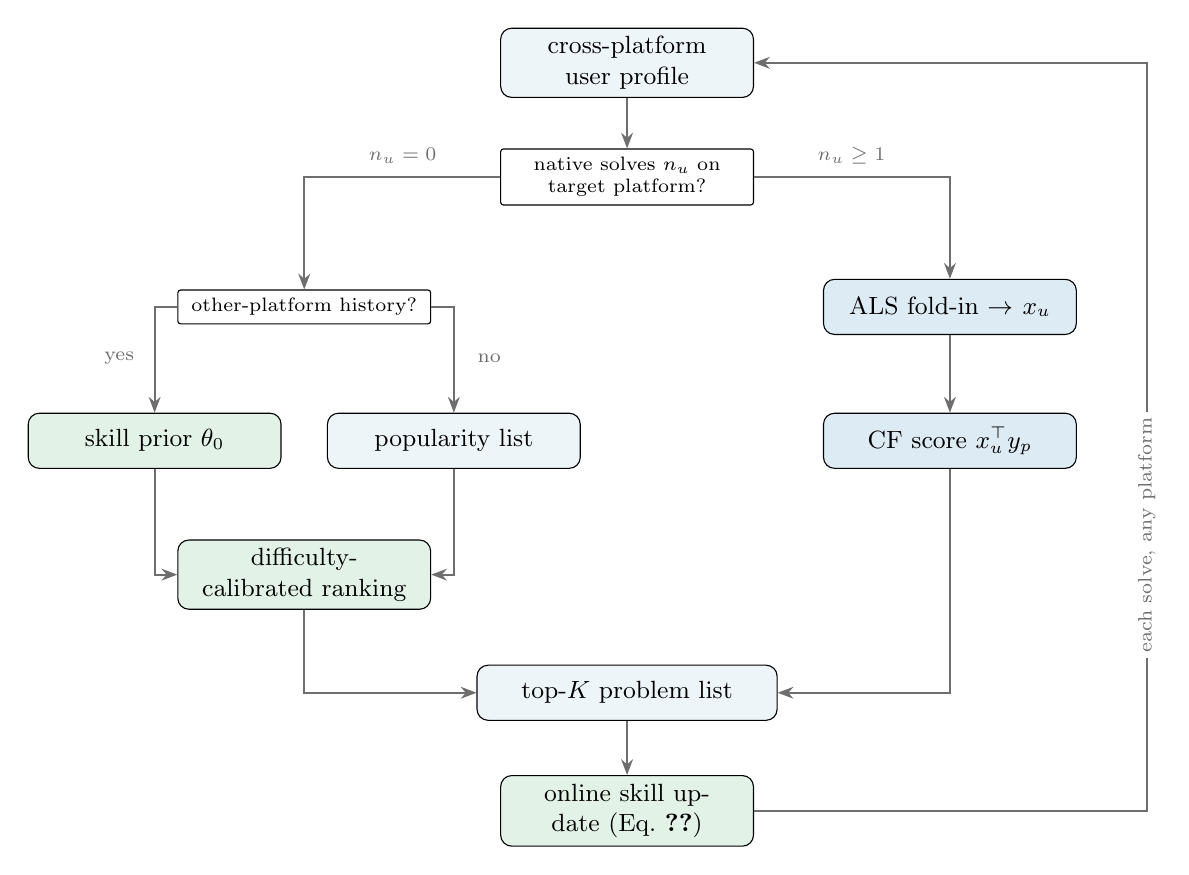
\begin{tikzpicture}[
    font=\small,
    box/.style={draw, rounded corners, align=center, inner sep=3pt,
                minimum height=7mm, text width=30mm, fill=cprsblue!8},
    warm/.style={box, fill=cprsblue!16},
    cold/.style={box, fill=cprsgreen!14},
    dec/.style={draw, rounded corners=1pt, align=center, font=\scriptsize,
                inner sep=3pt, text width=30mm, fill=white},
    arr/.style={-{Stealth[length=2mm]}, cprsgrey, thick},
    lbl/.style={font=\scriptsize, cprsgrey, inner sep=1.5pt}]

  \node[box] (prof) at (0,0)      {cross-platform user profile};
  \node[dec] (d1)   at (0,-1.45)  {native solves $n_u$ on target platform?};

  % ---- cold path (left) ----
  \node[dec]  (d2)    at (-4.1,-3.1) {other-platform history?};
  \node[cold] (prior) at (-6.0,-4.8) {skill prior $\theta_0$};
  \node[box]  (pop)   at (-2.2,-4.8) {popularity list};
  \node[cold] (rank)  at (-4.1,-6.5) {difficulty-calibrated ranking};

  % ---- warm path (right) ----
  \node[warm] (als) at (4.1,-3.1) {ALS fold-in $\to x_u$};
  \node[warm] (cfs) at (4.1,-4.8) {CF score $x_u^{\top} y_p$};

  \node[box, text width=36mm] (out) at (0,-8.0) {top-$K$ problem list};
  \node[cold] (upd) at (0,-9.5) {online skill update (Eq.~\ref{eq:skill})};

  \draw[arr] (prof) -- (d1);
  \draw[arr] (d1.west) -| (d2.north);
  \draw[arr] (d1.east) -| (als.north);
  \draw[arr] (d2.west) -| (prior.north);
  \draw[arr] (d2.east) -| (pop.north);
  \draw[arr] (prior.south) |- (rank.west);
  \draw[arr] (pop.south)   |- (rank.east);
  \draw[arr] (als) -- (cfs);
  \draw[arr] (rank.south) |- (out.west);
  \draw[arr] (cfs.south)  |- (out.east);
  \draw[arr] (out) -- (upd);

  % branch labels, placed explicitly to keep them off the routed lines
  \node[lbl] at (-2.85,-1.18) {$n_u=0$};
  \node[lbl] at ( 2.85,-1.18) {$n_u\geq1$};
  \node[lbl] at (-6.45,-3.75) {yes};
  \node[lbl] at (-1.75,-3.75) {no};

  % online correction loop, routed clear of every box on the right
  \draw[arr] (upd.east) -- ++(1.2,0) -- (6.6,-9.5) -- (6.6,0) -- (prof.east);
  \node[lbl, fill=white, inner sep=2pt] at (6.6,-6.0)
        {\rotatebox{90}{each solve, any platform}};
\end{tikzpicture}
\caption{Serving policy. The branch is on \emph{native} interaction count, so a user
experienced elsewhere but new here still takes the cold path --- where a cross-platform
skill prior is preferred to popularity. Every solve, on any platform, feeds the same
online skill estimate.}
\label{fig:policy}
\end{figure}

\subsection{Design Decisions and Alternatives}
Several decisions were made against alternatives and are worth recording. Template 1.1
(Data Science) was chosen over the web-design template because the project's centre of
gravity is the data pipeline and evaluation. For interaction data we chose to fetch from
the Codeforces API (sampling rated users) over downloading a large published dump, for
reproducibility and self-sufficiency. For difficulty we chose min--max normalisation over
an IRT calibration to keep the pipeline transparent, while explicitly testing the
resulting scale. For cross-platform value we \emph{began} with joint matrix factorisation
(the textbook approach) and only moved to a shared-ability model after the former failed
--- a decision the evaluation forced rather than anticipated.

%======================================================================
\section[Implementation \textnormal{\small(1,745 words)}]{Implementation}
\label{sec:impl}
%======================================================================

\subsection{Technology Stack and Software Structure}
The system is implemented in Python 3 across $32$ modules and approximately $5{,}200$
lines of code. Data science uses NumPy, SciPy (sparse matrices), scikit-learn (TF--IDF,
logistic regression, SVD) and the \texttt{implicit} library for ALS; the web application
uses FastAPI with a SQLite backend; figures use Matplotlib. Table~\ref{tab:structure}
summarises the layout.

\begin{table}[h]
\centering
\caption{Software structure. The pipeline is deliberately script-driven: each stage is a
separate entry point writing a versioned artefact, so any stage can be re-run in
isolation.}
\label{tab:structure}
\small
\begin{tabularx}{\textwidth}{@{}lrX@{}}
\toprule
\textbf{Package} & \textbf{Lines} & \textbf{Responsibility} \\
\midrule
\texttt{fetchers/} & 659 & One module per platform (Codeforces, AtCoder, CodeChef,
LeetCode); each exposes the same \texttt{fetch\_user\_submissions} interface, hiding four
very different APIs --- REST, community mirror, scraped HTML and GraphQL --- behind one
signature. \\
\texttt{models/} & 2{,}444 & Recommenders (\texttt{content}, \texttt{collaborative},
\texttt{hybrid}), the online skill estimator, the unified schema, cross-platform contest
normalisation and the serving engine. \\
\texttt{scripts/} & 4{,}122 & 27 stages: acquisition, dataset construction,
splitting, the six-model evaluation, significance testing, cold-start and
cross-platform studies, figures and reported statistics. \\
\texttt{app.py} & 286 & FastAPI application: auth, handle management, live
cross-platform profile assembly and the recommendation endpoint. \\
\bottomrule
\end{tabularx}
\end{table}

One structural decision did more work than any other. Every recommender implements the
same contract --- given a user index and the training matrix, return a dense score vector
over all candidate problems --- so the evaluation harness is model-agnostic. Adding
\texttt{diffmatch} as a fifth model during the investigation of the content result
(Section~\ref{sec:results}) required writing a scoring function and adding one name to a
list; no evaluation code changed. That uniformity is what made it cheap to keep asking
new questions of the data, and it is the main reason the comparison spans six models
rather than the two originally planned.

\subsection{Data Acquisition}
Problem catalogues are fetched once per platform. Codeforces submissions come from
\texttt{user.status}; AtCoder from the kenkoooo \texttt{/v3/user/submissions} endpoint,
paginated by timestamp; LeetCode from two public GraphQL queries. CodeChef is the
awkward case: its official API was withdrawn and now returns \texttt{401}, so the fetcher
uses the endpoints serving the site itself, reading the catalogue as JSON but
reconstructing histories from a submissions widget that yields a dozen HTML rows per
request and throttles an order of magnitude harder than the others. All fetchers enforce
a polite request delay and retry with exponential backoff, and write results
incrementally to JSON Lines so a long harvest is \emph{resumable} --- re-running skips
already-fetched users. Raw solve events are committed to disk so the exact dataset is
reproducible despite live API drift (a user's history grows over time).

\subsection{Interaction Dataset Construction}
\label{sec:impl-data}
We sample 3{,}000 rated Codeforces handles reproducibly (\texttt{user.ratedList}, fixed
seed) and fetch each user's full submission history, keeping accepted solves for problems
in the unified catalogue. An iterative $k$-core filter (retain users with $\geq5$ solves
and problems with $\geq5$ solvers, to a fixed point) removes noise and yields a sparse
implicit-feedback matrix of \textbf{2{,}459 users $\times$ 7{,}568 problems, 532{,}059
interactions} ($2.86\%$ density --- high for implicit feedback, a favourable CF signal).
A leave-last-$N$ temporal split (cap $10$, or $20\%$ per user, by solve time) yields
512{,}436 training and 19{,}623 test solves, with every user represented in both
(Figure~\ref{fig:pipeline}).

\begin{figure}[h]
\centering
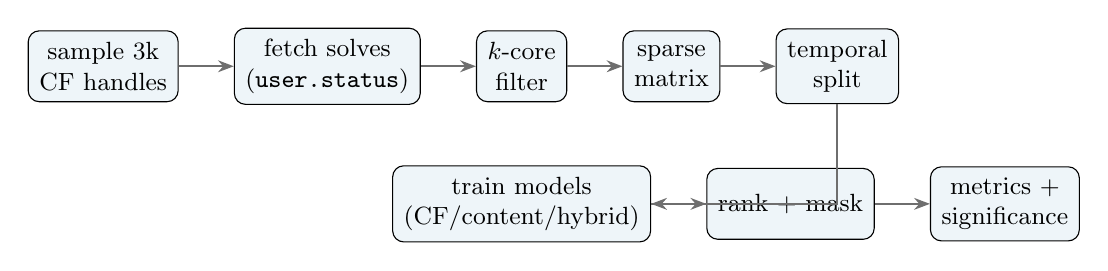
\begin{tikzpicture}[
    node distance=7mm,
    stage/.style={draw, rounded corners, align=center, minimum height=9mm,
                  font=\small, fill=cprsblue!8, inner sep=4pt},
    arr/.style={-{Stealth[length=2mm]}, cprsgrey, thick}]
  \node[stage] (a) {sample 3k\\CF handles};
  \node[stage, right=of a] (b) {fetch solves\\(\texttt{user.status})};
  \node[stage, right=of b] (c) {$k$-core\\filter};
  \node[stage, right=of c] (d) {sparse\\matrix};
  \node[stage, right=of d] (e) {temporal\\split};
  \node[stage, below=8mm of c] (f) {train models\\(CF/content/hybrid)};
  \node[stage, right=of f] (g) {rank + mask};
  \node[stage, right=of g] (h) {metrics +\\significance};
  \draw[arr] (a)--(b); \draw[arr] (b)--(c); \draw[arr] (c)--(d); \draw[arr] (d)--(e);
  \draw[arr] (e) |- (f); \draw[arr] (f)--(g); \draw[arr] (g)--(h);
\end{tikzpicture}
\caption{Data and evaluation pipeline, from API sampling to significance-tested metrics.}
\label{fig:pipeline}
\end{figure}

\subsection{Cross-Platform Cohort}
\label{sec:impl-cohort}
No directory links a user's identities across platforms, so we form a multi-platform
cohort by \emph{handle matching}: each Codeforces handle is probed on AtCoder, exploiting
the common practice of handle reuse. This yields \textbf{392 cross-platform users} and $\sim$30{,}000 AtCoder solves, of which
problems solved by $\geq3$ cohort members are retained as columns of a merged matrix.
Handle matching is a heuristic and is treated as a stated limitation
(Section~\ref{sec:threats}).

\subsection{Model Implementations}
\label{sec:impl-models}
The CF module wraps \texttt{implicit} ALS with $64$ factors, regularisation $0.05$, $20$
iterations and confidence scale $\alpha=15$ (Appendix~\ref{app:hyper}). Because
\texttt{implicit} needs a compiled native extension, the module carries a TruncatedSVD
fallback behind the same interface, so the pipeline degrades to a pure-Python path rather
than failing on a machine without a build toolchain --- which made the results reproduce
on a second machine unaided.

Three implementation details are worth setting out, because they are where the real
difficulty lay.

\paragraph{Vectorised scoring.} Scoring $2{,}459$ users against $7{,}568$ problems for six
models at three cut-offs is $\sim$$112$ million user--item evaluations per full run, and
the evaluation was re-run many times as the investigation developed. A per-user Python
loop over problems is hopelessly slow at that scale, so the content scorer precomputes
per-problem difficulty, log-popularity and a sparse problem$\times$tag matrix once, then
computes topic affinity for a whole batch of users as a single sparse matrix product;
the remaining difficulty-fit term is a vectorised Gaussian. CF scoring is a dense
$X Y^{\top}$ product. This turns a full six-model evaluation into a couple of minutes
rather than hours, which is what made the iterative, hypothesis-driven style of
Section~\ref{sec:results} practical at all.

\paragraph{Cold-start fold-in.} Simulating a user with only $k$ observed solves requires
a user factor that was \emph{not} learned during training, or the experiment leaks. We
therefore freeze the item factors $Y$ from the full fit and solve the ALS user-step in
isolation for the observed set $\mathcal{O}$:
\[
x \;=\; \big(\alpha\,Y_{\mathcal{O}}^{\top} Y_{\mathcal{O}} + \lambda I\big)^{-1}
        \alpha\,Y_{\mathcal{O}}^{\top}\mathbf{1},
\]
a $64\times64$ ridge system per probe user --- cheap enough ($O(f^3)$ with $f=64$, plus
$O(kf^2)$ to form the Gram matrix) to run for $1{,}976$ probe users across seven history
sizes. At $k=0$ the system degenerates to $x=0$, which is why CF scores collapse to a
constant and the model reduces to random ordering; this is a genuine property of the
method, not an artefact of the simulation.

\paragraph{The online skill estimator.} Equation~\ref{eq:skill} is implemented as a
$\sim$40-line class holding two floats. \texttt{update()} is a single comparison and one
addition --- $O(1)$ per solve with $O(1)$ memory, so it can run in the request path --- while
\texttt{seed()} initialises $\theta$ to the empirical $q$-quantile of \emph{any} supplied
difficulty history, which is the mechanism by which an AtCoder history becomes a
Codeforces prior. Because both entry points write the same state, seeding and live correction compose
without special-casing: the \texttt{atcoder+cf\_5} condition of
Section~\ref{sec:results-xplat} is a \texttt{seed()} call followed by five
\texttt{update()} calls. The estimate is clipped to $[0,1]$.

\subsection{Web Application}
\label{sec:impl-web}
A FastAPI application serves the system live, exposing session and registration
endpoints, platform-handle management, recommendation and catalogue statistics. A
SQLite schema (Figure~\ref{fig:er}) stores \texttt{users} (salted SHA-256 password
hashes), \texttt{platform\_handles} and \texttt{sessions} (cookie tokens); the credential
database is never committed. The schema is deliberately minimal, and the reason is a
design position rather than an omission: CPRS stores \emph{identity}, not behaviour. A
user's solve history is re-fetched from the origin platforms on demand rather than
mirrored locally, so the application holds no copy of anyone's submission record, cannot
drift out of date with the judges, and has nothing to leak beyond a handle that is
already public.

\begin{figure}[h]
\centering
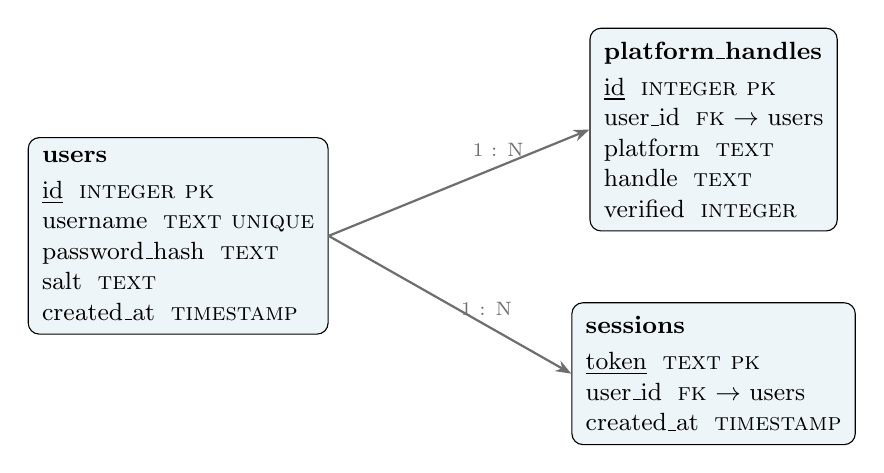
\begin{tikzpicture}[
    font=\small,
    ent/.style={draw, rounded corners, align=left, inner sep=5pt, fill=cprsblue!8},
    arr/.style={-{Stealth[length=2mm]}, cprsgrey, thick},
    lbl/.style={font=\scriptsize, cprsgrey}]

  \node[ent] (u) at (0,0) {%
    {\bfseries users}\\[2pt]
    \underline{id} \;\textsc{integer pk}\\
    username \;\textsc{text unique}\\
    password\_hash \;\textsc{text}\\
    salt \;\textsc{text}\\
    created\_at \;\textsc{timestamp}};

  \node[ent] (h) at (6.8,1.35) {%
    {\bfseries platform\_handles}\\[2pt]
    \underline{id} \;\textsc{integer pk}\\
    user\_id \;\textsc{fk} $\to$ users\\
    platform \;\textsc{text}\\
    handle \;\textsc{text}\\
    verified \;\textsc{integer}};

  \node[ent] (s) at (6.8,-1.75) {%
    {\bfseries sessions}\\[2pt]
    \underline{token} \;\textsc{text pk}\\
    user\_id \;\textsc{fk} $\to$ users\\
    created\_at \;\textsc{timestamp}};

  \draw[arr] (u.east) -- node[lbl, above, pos=0.65] {1 : N} (h.west);
  \draw[arr] (u.east) -- node[lbl, above, pos=0.65] {1 : N} (s.west);
\end{tikzpicture}
\caption{Database schema. Only identity is persisted --- solve histories are re-fetched
from the origin platforms on each request rather than mirrored.}
\label{fig:er}
\end{figure}

On a
recommendation request the app fetches the user's recent submissions across their linked
platforms, merges them into a single profile (unioning solved sets, combining per-topic
mastery, taking the max rating), analyses recent-performance trend, and returns ranked
recommendation cards with platform badges, difficulty, topic tags and a direct link to
the origin judge. Because the user solves on the native judge and new submissions are picked up on the
next refresh, no submission proxying is required.

\subsection{Reproducibility and Engineering Practice}
Every result in this report is regenerable from committed raw data by a fixed sequence of
scripts (Appendix~\ref{app:repro}); random seeds are fixed for sampling, ALS and
bootstrap. Derived artefacts (matrices, splits, metrics, figures) are produced
deterministically, and the decisions log records the rationale and results of each major
step as the project progressed. Freezing the raw solve events on disk matters more here
than it might elsewhere: a Codeforces user's history grows continuously, so an evaluation
that re-fetched from the API would silently change its own test set between runs and no
two numbers in this report would be comparable.

\subsection{Verification and Correctness}
\label{sec:impl-testing}
Correctness in a pipeline of this kind is mostly a question of whether a surprising number
is a finding or a bug. Two things guard against the second possibility: an automated test
suite over the components where a silent error would be least visible, and a set of
working habits around surprising results.

\paragraph{Automated tests.} A \texttt{pytest} suite of $126$ tests covers seven areas
(Table~\ref{tab:tests}). The choice of targets is deliberate. An error in the ranking
metrics --- a wrong \ndcg{} denominator, an off-by-one in the rank of the first hit ---
would scale every model by the same factor and so would \emph{not} disturb the model
ordering on which the report's conclusions rest; it would be invisible to inspection but
would falsify every absolute number. The metric definitions are therefore pinned to
arithmetic worked by hand. Likewise, a leak between train and test would inflate all
models together, so the split's integrity is asserted directly against the committed
artefacts rather than a synthetic fixture: no held-out item appears in any user's
training row, train and test exactly partition the full matrix, and the $k$-core has
genuinely reached a fixed point.

\begin{table}[h]
\centering
\caption{Test suite. The dataset tests run against the committed artefacts, so they
verify the data the results are actually computed on.}
\label{tab:tests}
\small
\begin{tabularx}{\textwidth}{@{}lrX@{}}
\toprule
\textbf{Module} & \textbf{Tests} & \textbf{What is asserted} \\
\midrule
\texttt{test\_contests.py} & 35 & Rating-history normalisation for each platform's
payload shape; delta reconstruction where only post-contest ratings are published;
trend, volatility and calibration confidence. \\
\texttt{test\_codechef.py} & 35 & Sentinel difficulties rejected rather than normalised
to zero; the taxonomy used as a whitelist so setter usernames are discarded; submission
rows parsed from the cell attribute rather than the intermittent link; statement
extraction degrading rather than raising on malformed author markup. \\
\texttt{test\_metrics.py} & 14 & \ndcg{}/MRR/precision/recall/hit against hand-computed
values; the \ndcg{} denominator's $\min(|\mathcal{R}|,K)$ convention; masking of
already-solved items; monotonicity in $K$. \\
\texttt{test\_skill.py} & 13 & Convergence in mean to the $q$-quantile; no upward drift
on solve-only data; seed-then-correct composition; clipping; tolerance of missing
difficulties. \\
\texttt{test\_foldin.py} & 12 & Fold-in shape and determinism; that a folded-in user
reproduces the batch-trained factors for an unchanged history. \\
\texttt{test\_dataset.py} & 9 & $k$-core fixed point; binary implicit feedback; no
train/test leakage; train $+$ test partitions the matrix; every user present in both;
metadata agrees with the artefacts. \\
\texttt{test\_topic\_targeting.py} & 8 & Weak-topic selection; that absent tags are not
read as evidence of weakness across platform vocabularies. \\
\bottomrule
\end{tabularx}
\end{table}

Writing the tests was not merely confirmatory. The skill estimator's convergence test
initially failed, informatively: with a \emph{constant} step size the estimate does not
converge pointwise to the $q$-quantile but performs a random walk whose stationary
\emph{mean} is the quantile. The instantaneous estimate therefore carries a noise floor
proportional to $\eta$ --- about $0.04$ on the $[0,1]$ scale at the deployed $\eta=0.02$,
against $0.007$ at $\eta=0.001$. The seeded estimates of Section~\ref{sec:results-xplat}
are unaffected (\texttt{seed()} sets the quantile exactly), but the purely online
estimate should be read as a running average, not a point value --- a property we would
not have stated without trying to assert it.

\paragraph{Working habits.} Four practices did the rest.
\emph{Baselines as assertions.} A \texttt{random} model runs in every experiment as a
lower-bound check. Its scores sit exactly where theory puts them (\ndcg{}@10 $=0.0012$,
$\approx K/|\mathcal{C}|$ for HitRate@$K$) --- a continuous signal that ranking, masking
and metric code are not silently broken. \emph{Leakage checks.} Training solves are
masked before ranking, and fold-in uses item factors fitted without the probe user's
held-out items; the $k=0$ degeneracy ($x=0$) was traced analytically to confirm it was
the method's behaviour, not an indexing error. \emph{Adversarial re-testing of
surprises.} Both counter-intuitive results were re-examined before being believed: the
content model's chance-level performance was diagnosed with an opposed scorer
(\texttt{diffmatch}) that moved the metric five-fold in the predicted direction, and the
cross-platform transfer failure was re-tested under three independent designs. \emph{Regenerability as a regression test.} Because the
whole pipeline is deterministic under fixed seeds, re-running it after a change and
diffing the metric JSON detects unintended effects; the statistics quoted in this report
are themselves regenerated by \texttt{report\_stats.py} rather than transcribed, which
caught two figures that had drifted from the data during drafting.

The suite's limits should be stated plainly. It covers the metric, split, skill and
normalisation components, and the parsers that turn each platform's payload into the
unified schema, but not live fetching (which would need recorded API fixtures), the ALS
wrapper (whose numerical behaviour is the upstream library's) or the web layer (which has
no endpoint tests). Coverage is therefore concentrated where a silent failure would be both plausible and
invisible, rather than uniform; a system maintained by others would need the rest.

%======================================================================
\section[The NLP Cross-Platform Auto-Tagger \textnormal{\small(755 words)}]{The NLP Cross-Platform Auto-Tagger}
\label{sec:tagger}
%======================================================================

\subsection{Motivation}
AtCoder publishes \emph{no} topic tags. Its problems do carry labels, but they are
contest-series identifiers (\texttt{abc}, \texttt{arc}) that say when a problem was set,
not what it is about; measured against the canonical taxonomy, topic coverage on AtCoder
is exactly $0\%$ of $9{,}095$ problems, against $96.2\%$ on Codeforces and $88.6\%$ on
LeetCode. Over half the unified catalogue ($25{,}342$ problems, $55.2\%$) carries no usable topic
metadata, and it is not a random half --- it is concentrated in two platforms. Topic-gap
recommendation and cross-platform topic comparison are impossible on that slice unless
the tags are inferred. We frame this as cross-platform \emph{label} transfer: exploit a
richly-labelled platform to annotate an unlabelled one. The task is a close relative of
Zhao et al.'s~\cite{zhao2018} recovery of topics and difficulty from submission logs,
but uses the complementary signal --- the problem statement itself.

\subsection{Approach}
A multi-label classifier is trained on Codeforces problem statements, which carry
human-curated tags, and applied to AtCoder statements. Text is vectorised with TF--IDF
($10\,000$ features, bigrams, sublinear term frequency) and classified with one-vs-rest
$\ell_2$-regularised logistic regression with balanced class weights. Training uses
$1{,}999$ scraped Codeforces statements; inference targets $795$ AtCoder statements that
were reachable ($4{,}205$ were blocked by the platform's anti-scraping protections --- a
limitation discussed below). Performance is estimated by $5$-fold cross-validation on the
Codeforces set.

\subsection{Cross-Validation Results}
Micro-averaged $F_1$ is $0.53$ and macro-averaged $F_1$ is $0.44$ across sixteen
frequent tags. Table~\ref{tab:tagger} shows the per-tag breakdown for a representative
selection; the spread is large and systematic, which is the interesting part.

\begin{table}[h]
\centering
\caption{Per-tag $5$-fold cross-validation of the NLP tagger (selected tags, sorted by
$F_1$). ``Content'' tags with distinctive vocabulary are learnable; ``method'' tags that
describe a solution technique are not.}
\label{tab:tagger}
\small
\begin{tabular}{lcccc}
\toprule
tag & type & precision & recall & $F_1$ \\
\midrule
strings              & content & 0.64 & 0.86 & 0.74 \\
math                 & content & 0.67 & 0.72 & 0.69 \\
greedy               & content & 0.65 & 0.68 & 0.66 \\
implementation       & content & 0.58 & 0.60 & 0.59 \\
dfs                  & mixed   & 0.53 & 0.34 & 0.41 \\
sorting              & mixed   & 0.31 & 0.41 & 0.35 \\
data\_structures     & method  & 0.24 & 0.28 & 0.26 \\
binary\_search       & method  & 0.25 & 0.24 & 0.25 \\
dynamic\_programming & method  & 0.24 & 0.17 & 0.20 \\
two\_pointers        & method  & 0.19 & 0.18 & 0.18 \\
\bottomrule
\end{tabular}
\end{table}

\subsection{Threshold Calibration}
Predicted probabilities are thresholded before display. Sweeping a global threshold by
$5$-fold CV, $F_1$ peaks at $0.5$ (precision $0.51$, recall $0.54$, $2.5$ tags on
average); per-tag thresholds (Appendix~\ref{app:hyper}) improve individual tags further.
Displayed tags are always labelled ``predicted'' or ``curated'', so provenance is
transparent.

\subsection{The Two-Tier Finding}
The per-tag results reveal a clean dichotomy that is a contribution in its own right.
\emph{Content} tags (\texttt{strings}, \texttt{math}, \texttt{game\_theory}) score highly
because they correspond to distinctive statement vocabulary. \emph{Method} tags
(\texttt{dynamic\_programming}, \texttt{binary\_search}) score poorly because they describe
\emph{how} to solve a problem, not \emph{what} it says: a DP problem may be dressed as a
grid, a sequence or a game, so its text does not reliably signal the technique. Text-based tagging is therefore intrinsically limited for
method tags, and a stronger tagger would need structural features (difficulty, solve
rate, editorial signals), not just text. On the reachable AtCoder problems the tagger
assigns tags to $775/795$ ($97.5\%$), averaging $1.9$ tags each, with the predicted
distribution dominated by content tags as expected.

\subsection{Limitations}
The honest headline is that the method works better than its deployment does. Only $16\%$
of targeted AtCoder pages were reachable behind the platform's anti-scraping protections,
so although the tagger labels $97.5\%$ of the statements it can see, catalogue-level
AtCoder topic coverage rises only from $0\%$ to $8.5\%$ ($775$ of $9{,}095$ problems).
The bottleneck is therefore \emph{corpus access}, not modelling: a production system
would use a cached statement corpus (e.g.\ IBM CodeNet) or authenticated, throttled
access, and the same trained model would then annotate the remaining $8{,}320$ problems
without any change. Section~\ref{sec:tagger-codechef} tests that claim directly on a
platform that does grant access. A second limitation is intrinsic rather than logistical --- the
two-tier finding above means that even with full corpus access, method tags would remain
poorly recovered from text alone. Finally, the tagger is confined to the sixteen most
frequent tags, below which Codeforces training support becomes too thin to estimate a
reliable decision threshold; rarer topics would need either more training data or a
hierarchical model that borrows strength from related tags. A knock-on consequence for
the wider project is that AtCoder difficulty, too, is incomplete: only $51.7\%$ of
AtCoder problems carry a community difficulty estimate, which bounds how much of that
platform the difficulty-matching scorer can reach.

\subsection{A Second Target Platform}
\label{sec:tagger-codechef}
The claim above --- that the ceiling was corpus \emph{access}, not modelling --- needs a
platform that grants it, and CodeChef serves statements as structured JSON. The same
trained model, unchanged, was pointed at it. All $5{,}520$ rated problems were retrieved:
$100\%$ corpus reach against AtCoder's $16\%$. The model tagged $1{,}480$ problems
CodeChef had left unlabelled, lifting canonical-topic coverage from $3{,}950$ to
$5{,}430$. The diagnosis holds: given access, the untouched model annotates almost
everything it sees. Catalogue coverage stays at $25.2\%$ only because one request per
problem puts the full $21{,}568$ at twelve hours of polite fetching --- a budget, not a
barrier, and exactly the distinction AtCoder could not settle.

%======================================================================
\section[Evaluation Methodology \textnormal{\small(1,147 words)}]{Evaluation Methodology}
\label{sec:eval}
%======================================================================

The evaluation has to answer a specific question --- \emph{would this system have put the
right problem in front of this user?} --- and every choice below follows from taking that
question literally rather than from convention.

\subsection{Dataset and Protocol}
All ranking results are on the held-out temporal test set of the $2{,}459$-user matrix
(Section~\ref{sec:impl-data}). Each user's most-recent solves are the test set; models
rank all $7{,}568$ candidate problems with the user's training solves masked out, and are
scored on whether the held-out problems surface near the top.

\paragraph{Why a temporal split.} A random hold-out would let a model be trained on a
user's March solves and tested on their January ones. That is not the deployed task: in
deployment the entire future is unavailable, and recommending a problem the user has
already outgrown is a failure the metric would silently reward. Splitting on solve time
reproduces the real information boundary, which is why the recommender-systems literature
treats it as the more faithful protocol~\cite{cremonesi2010}. It also makes the task
strictly harder --- and is one reason the absolute numbers here are lower than
single-platform studies using random splits typically report.

\paragraph{Why leave-last-$N$ rather than a global time cut.} A single global cut-off date
would give heavy users a large test set and users who stopped early none at all, so the
evaluated population would silently become ``users active in the final window''. Holding
out each user's own last $\min(10, 20\%)$ solves keeps all $2{,}459$ users in the
evaluation, keeps per-user test sizes comparable (mean $7.98$), and asks the same question
of every user regardless of when they were active.

\paragraph{Why masking matters.} Training solves are removed from every model's candidate
list before ranking. Without this, a model could score highly by recommending what a user
has already done --- trivially predictable and useless --- and CF in particular would be
flattered, since factorisation reconstructs observed entries by construction.

\paragraph{What this protocol cannot measure.} It is worth being explicit that next-solve
prediction is a \emph{proxy}. It measures agreement with what users did, not whether what
they did was good for them, so a recommender that perfectly predicted a learner's
unproductive habits would score perfectly. Nothing in this evaluation can distinguish a
useful recommendation from a merely accurate one, and Section~\ref{sec:threats} treats
this as the study's principal threat to validity rather than a footnote.

\subsection{Metrics}
For a user with held-out set $\mathcal{R}$ and top-$K$ recommendation list $\mathcal{L}_K$
(best first), we report, averaged over users:
\begin{align*}
\text{HitRate@}K &= \mathbb{1}[\mathcal{L}_K \cap \mathcal{R} \neq \varnothing], &
\text{Precision@}K &= \frac{|\mathcal{L}_K \cap \mathcal{R}|}{K}, \\
\text{Recall@}K &= \frac{|\mathcal{L}_K \cap \mathcal{R}|}{|\mathcal{R}|}, &
\text{MRR@}K &= \frac{1}{\text{rank of first hit}},
\end{align*}
and normalised discounted cumulative gain
\[
\text{\ndcg{}@}K = \frac{\sum_{i=1}^{K} \mathrm{rel}_i/\log_2(i+1)}
{\sum_{i=1}^{\min(|\mathcal{R}|,K)} 1/\log_2(i+1)},
\]
at $K\in\{5,10,20\}$, with $\mathrm{rel}_i\in\{0,1\}$ indicating whether the item at
rank $i$ is relevant.

The five are reported together because each is blind to something the others see.
HitRate answers the product question --- did the user get \emph{anything} useful? --- but
cannot tell one hit from five. Precision and Recall trade against each other and are both
distorted by variable test-set sizes: with $|\mathcal{R}|$ capped at $10$ but often
smaller, Precision@10 is bounded by $|\mathcal{R}|/10$. MRR captures only the first hit,
which matters for a short list but ignores everything below it. \ndcg{} is our headline metric because it is the only one of the five that is
sensitive to \emph{both} how many relevant items appear and where they appear, via the
$1/\log_2(i+1)$ discount --- the right shape for a ranked list a user reads from the top.
Reporting all five at three cut-offs also guards against a conclusion that holds only at
one arbitrary $K$; Figure~\ref{fig:metrick} confirms the model ordering is stable across
cut-offs, which is the check that licenses quoting $K=10$ throughout.

One consequence deserves flagging, because it affects how the results table should be
read: all five metrics are computed per user and then averaged unweighted, so a user with
$200$ training solves counts exactly as much as one with $5$. This is right for a system judged on its service to individuals rather than aggregate
traffic, but it means the headline numbers are not dominated by heavy users --- and since
those are the hardest to predict (Section~\ref{sec:results}), the averages sit lower than
an interaction-weighted alternative would give.

\subsection{Models and Baselines}
Seven models are compared, and the set is constructed so that each one isolates a
specific claim rather than merely adding a row to the table.

\texttt{random} is a lower bound that doubles as a live correctness check: its scores are
predictable in closed form, so if the harness were mis-wired, random would not land where
arithmetic says it should (Section~\ref{sec:impl-testing}). \texttt{popularity} is the
non-personalised reference the literature identifies as deceptively hard to
beat~\cite{cremonesi2010}; including it is what makes ``CF is good'' a meaningful claim
rather than an unfalsifiable one, since any personalised model that cannot beat
popularity has demonstrated nothing. \texttt{content} (pedagogical) and \texttt{diffmatch}
(difficulty-matching) are a matched pair, deliberately opposed on both of the axes that
define the content scorer --- unseen versus familiar topics, stretch versus at-level
difficulty. Comparing them turns a puzzling result into a diagnosis: if content's failure
is caused by that design stance rather than by a defect, reversing the stance must move
the metric, and by how much is itself evidence. \texttt{cf} (ALS) is the personalised
model under test, and the two hybrids (\texttt{hybrid} $=$ CF$+$content,
\texttt{hybrid\_pop} $=$ CF$+$popularity) test whether blending helps at all and, by
differing only in the cold ingredient, separate ``blending is wrong'' from ``this
particular ingredient is weak''.

\subsection{Significance and Uncertainty}
Per-user \ndcg{}@10 is strongly non-normal and zero-inflated --- a spike at zero with a
thin right tail, since most users receive no hit --- which rules out a $t$-test on the raw
scores. We therefore test model differences with the paired Wilcoxon signed-rank
test~\cite{wilcoxon1945}, which compares the \emph{same} users under two models and so
removes the between-user variance that would otherwise swamp the model effect.

Significance alone is uninformative at this sample size: with $n=2{,}459$ paired
observations, differences far too small to matter clear any conventional threshold.
We therefore report a rank-biserial effect size alongside every $p$-value, and bootstrap
($2{,}000$-resample) $95\%$ confidence intervals on each model's mean, so results read as
intervals rather than points. This combination --- paired non-parametric test, effect size, and intervals against a
strong baseline --- is what Dacrema et al.~\cite{dacrema2019} find missing from much of
the recommender literature, and following it is part of why two headline findings here
are negative.

\subsection{Cold-Start and Cross-Platform Designs}
Cold start is probed with a \emph{fold-in simulation}: using fixed item factors from the
full fit, we reveal only a user's $k$ most-recent solves, solve
$\;\big(\alpha Y_{\mathcal{O}}^\top Y_{\mathcal{O}} + \lambda I\big)x = \alpha Y_{\mathcal{O}}^\top\mathbf{1}$
for their folded factor $x$, and evaluate as $k$ varies. The cross-platform questions use
three designs on the cohort: (A) train CF-only vs.\ CF+AtCoder and compare CF-side quality
at full history; (B) neighbourhood transfer (recommend what AtCoder-similar users solved
on CF) for a zero-CF-history user; and the skill experiments of
Section~\ref{sec:results-xplat}.

%======================================================================
\section[Results \textnormal{\small(885 words)}]{Results}
\label{sec:results}
%======================================================================
This section is written as an inquiry: each subsection poses a hypothesis, tests it, and
--- where the data demands --- refutes and refines it.

\subsection{RQ1: Which paradigm predicts next solves?}
Table~\ref{tab:overall} and Figure~\ref{fig:modelcmp} give the headline comparison.
Collaborative filtering is decisively best: \ndcg{}@10 $=0.096$ and HitRate@10 $=0.295$
--- nearly one user in three receives a genuine next-solve in their top ten --- roughly
$2\times$ popularity and $26\times$ random. Every difference from CF is significant (paired
Wilcoxon on per-user \ndcg{}@10): versus popularity $p=6\times10^{-43}$ with a
medium--large effect ($r=0.45$); versus the hybrids $p<10^{-2}$. Bootstrap $95\%$ CIs
(Figure~\ref{fig:modelcmp}) separate CF from popularity.

\begin{table}[h]
\centering
\caption{Overall ranking quality on the held-out temporal test ($2{,}459$ users). Best per
column in bold.}
\label{tab:overall}
\small
\begin{tabular}{lccccc}
\toprule
model & HitRate@10 & Prec@10 & Recall@10 & MRR@10 & \ndcg{}@10 \\
\midrule
random      & 0.0114 & 0.0011 & 0.0014 & 0.0035 & 0.0012 \\
content     & 0.0094 & 0.0009 & 0.0015 & 0.0030 & 0.0012 \\
diffmatch   & 0.0407 & 0.0044 & 0.0048 & 0.0198 & 0.0061 \\
popularity  & 0.1440 & 0.0230 & 0.0429 & 0.0651 & 0.0374 \\
hybrid      & 0.2908 & 0.0577 & 0.1007 & 0.1178 & 0.0810 \\
hybrid\_pop & 0.2985 & 0.0588 & 0.1133 & 0.1261 & 0.0901 \\
\textbf{cf} & \textbf{0.2952} & \textbf{0.0593} & \textbf{0.1180} & \textbf{0.1304} & \textbf{0.0959} \\
\bottomrule
\end{tabular}
\end{table}

\begin{figure}[h]
\centering
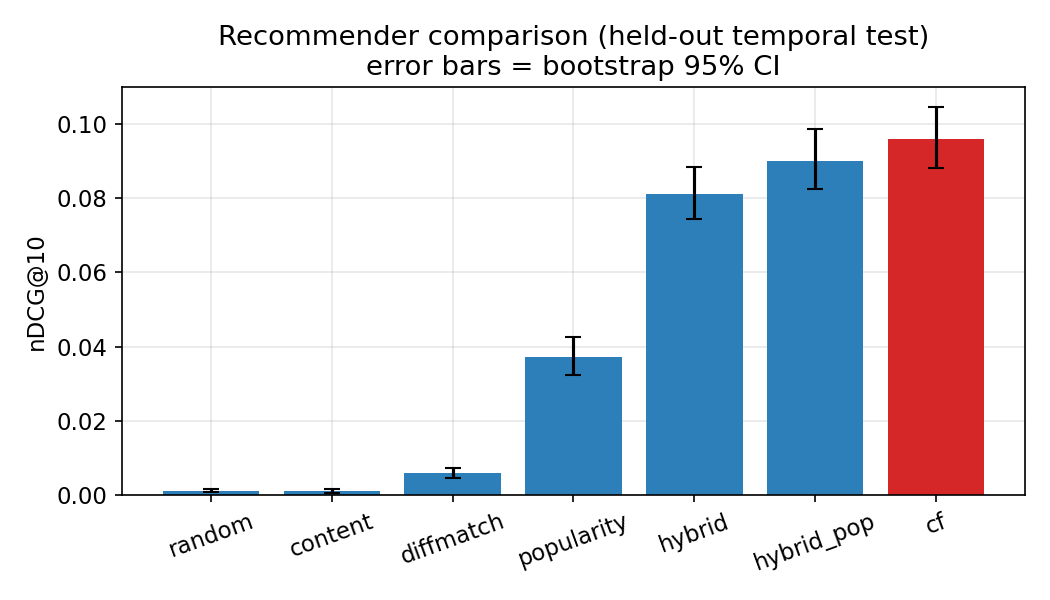
\includegraphics[width=0.7\textwidth]{figures/model_comparison.png}
\caption{Model comparison on \ndcg{}@10 with bootstrap $95\%$ confidence intervals. CF
(red) is significantly best; content and difficulty-matching are poor \emph{ranking}
predictors.}
\label{fig:modelcmp}
\end{figure}

Two findings deserve emphasis. First, the pedagogical \texttt{content} model performs at
chance ($0.0012$, indistinguishable from \texttt{random}). This is not a defect: it
recommends \emph{unseen} topics at \emph{stretch} difficulty --- pedagogically sensible
but anti-correlated with what users actually do next, which is to continue in familiar
topics near their level. Re-aiming it to at-level, familiar problems (\texttt{diffmatch})
raises \ndcg{}@10 five-fold to $0.0061$, confirming the diagnosis, though it stays far
below CF because hundreds of problems fit any difficulty/topic band and predicting the
\emph{exact} next one is intrinsically hard. Figure~\ref{fig:metrick} shows the ordering is
stable across cut-off $K$.

\subsection{A hypothesis refuted: the hybrid does not win}
We expected a hybrid to be the strongest model. It is not: \texttt{hybrid}
($0.081$) and \texttt{hybrid\_pop} ($0.090$) both fall \emph{below} pure CF ($0.096$),
significantly so. The explanation is structural: the $k$-core-filtered matrix contains no
genuinely cold users (every user has $\geq5$ solves), so CF already has sufficient signal
for everyone in it, and blending in a weaker ingredient only dilutes it. This is the
first point at which the data redirected the project: if the hybrid's value is to appear
anywhere, it must be at true cold start --- which this test set does not contain, and which
we therefore simulate next.

\begin{figure}[h]
\centering
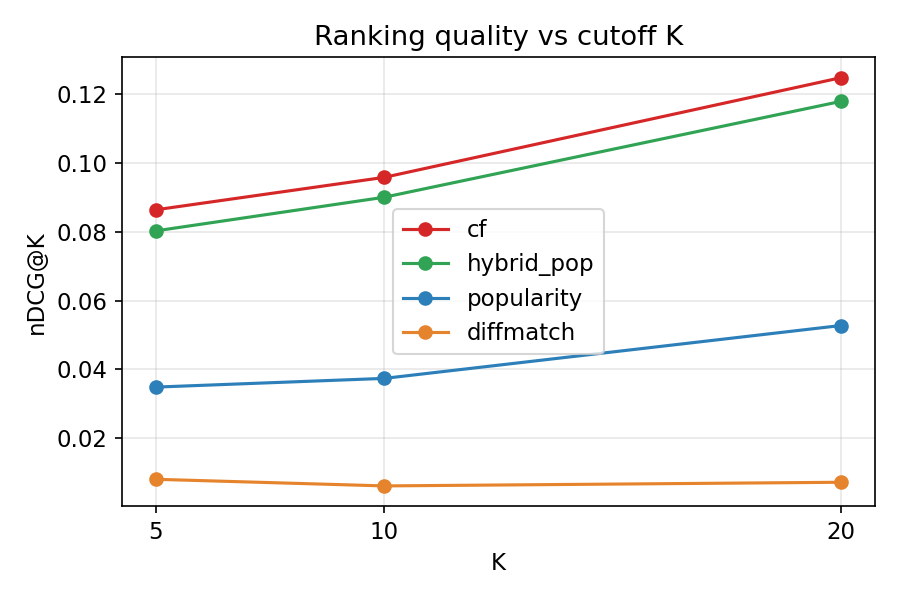
\includegraphics[width=0.58\textwidth]{figures/metric_vs_k.png}
\caption{\ndcg{}@$K$ across cut-offs; the model ordering is stable.}
\label{fig:metrick}
\end{figure}

\subsection{RQ2: Cold-start behaviour}
Slicing by activity (Figure~\ref{fig:buckets}) shows CF leading in every bucket, but with
both its advantage and the absolute scores falling for high-activity users, whose recent
solves are rare, advanced problems that are intrinsically hard to predict. To reach the
true cold-start regime we run the fold-in simulation (Figure~\ref{fig:coldstart}): at
$k=0$ CF collapses to random ($0.001$) and popularity wins ten-fold; from $k=1$ CF fold-in
dominates --- a single interaction is enough to place a user usefully in latent space. The
evidence-driven policy is therefore a \emph{near-hard switch} --- a non-personalised (or,
better, cross-platform) prior for zero-history users, personalised CF from the first solve
--- rather than the slow density ramp we originally designed. The smooth hybrid was solving
a problem the data does not pose.

\begin{figure}[h]
\centering
\begin{minipage}{0.49\textwidth}\centering
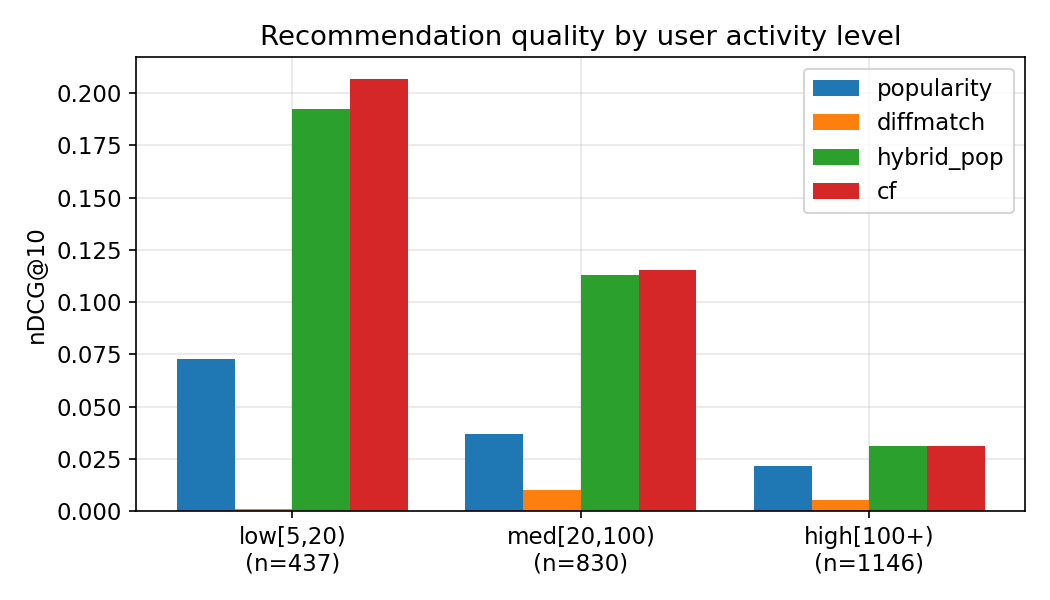
\includegraphics[width=\textwidth]{figures/activity_buckets.png}
\caption{\ndcg{}@10 by user-activity bucket.}
\label{fig:buckets}
\end{minipage}\hfill
\begin{minipage}{0.49\textwidth}\centering
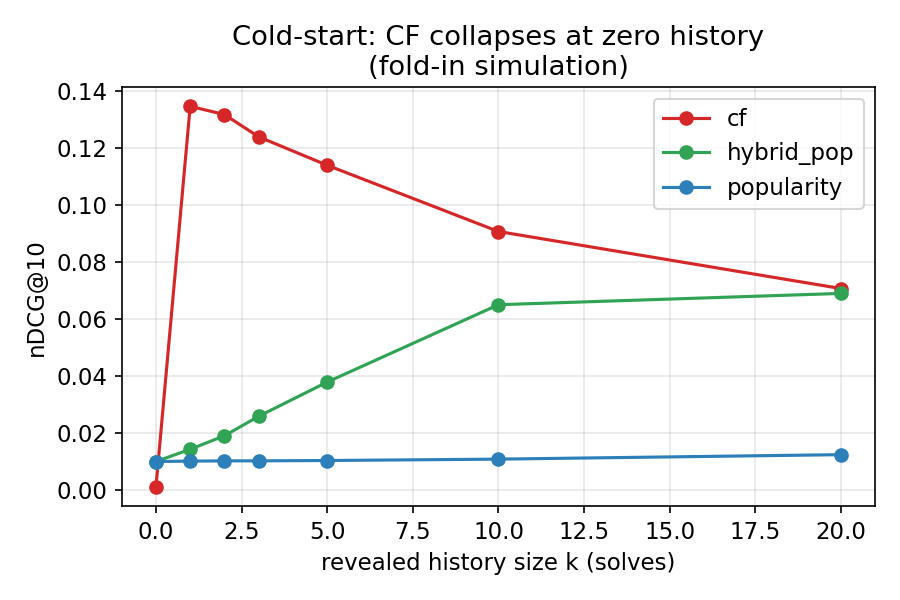
\includegraphics[width=\textwidth]{figures/coldstart_curve.png}
\caption{Cold-start fold-in: CF collapses at $k=0$, dominates from $k=1$.}
\label{fig:coldstart}
\end{minipage}
\end{figure}

\subsection{RQ3: Does cross-platform \emph{collaborative} transfer help?}
\label{sec:results-xplat}
With cold start pinpointed, the project's central premise becomes concrete: a user new to
Codeforces but experienced on AtCoder should be rescuable by their cross-platform history.
We tested this the textbook way first --- joint matrix factorisation --- and it failed.
Table~\ref{tab:xplat} (Design~A) shows that training ALS on the merged CF+AtCoder matrix
leaves full-history CF quality essentially unchanged ($0.038$ vs.\ $0.039$), and folding a
user in with their AtCoder items actively \emph{hurts} at low history ($0.033$ vs.\ $0.089$
\ndcg{}@10 at $k=1$; Design~B, not shown). The reason is exactly the cross-domain warning
of Section~\ref{sec:lit}: AtCoder problems are solved only by the small cohort, so their
latent factors occupy a subspace weakly aligned with the CF factors, and importing them
drags the user vector away from the CF-relevant region. A lighter neighbourhood-transfer
variant does beat popularity roughly two-fold for a zero-history user
($0.0053$ vs.\ $0.0027$ \ndcg{}@10), but remains far below the value of a single native
solve.

\begin{table}[h]
\centering
\caption{Design~A --- cross-platform value for full-history cohort users ($n=382$).
Merging AtCoder history does not improve CF-side recommendation.}
\label{tab:xplat}
\small
\begin{tabular}{lccc}
\toprule
training data & \ndcg{}@10 & HitRate@10 & Recall@10 \\
\midrule
CF only            & 0.0393 & 0.1545 & 0.0439 \\
CF + AtCoder (cross) & 0.0380 & 0.1492 & 0.0398 \\
\bottomrule
\end{tabular}
\end{table}

A second, sharper refutation followed. The population the premise targets --- new to
Codeforces yet experienced elsewhere --- is \emph{empirically rare}: of $247$ held-out
low-CF-activity users, \emph{none} had substantial AtCoder history, because handle-matched
multi-platform users are, almost by definition, experienced on every platform they use.
Naive collaborative transfer across disjoint problem sets thus offers little here, both
mechanically and demographically.

\subsection{RQ4: Skill transfers --- the pivot}
At this point the premise looked dead. The recovery came from asking a different question:
perhaps what transfers across platforms is not item co-occurrence but \emph{ability}.
Figure~\ref{fig:scatter} plots, for $186$ users active on both platforms, their Codeforces
skill against their AtCoder skill (75th-percentile normalised difficulty solved). The two
correlate strongly --- \textbf{Pearson $r=0.77$} ($p\approx4\times10^{-38}$; Spearman
$\rho=0.75$), with matched means ($0.247$ vs.\ $0.260$). Skill is a property of the
\emph{person}, and the unified difficulty scale makes it comparable; this simultaneously
validates the normalisation of Section~\ref{sec:design-data} and explains why skill
transfers where items do not.

\begin{figure}[h]
\centering
\begin{minipage}{0.46\textwidth}\centering
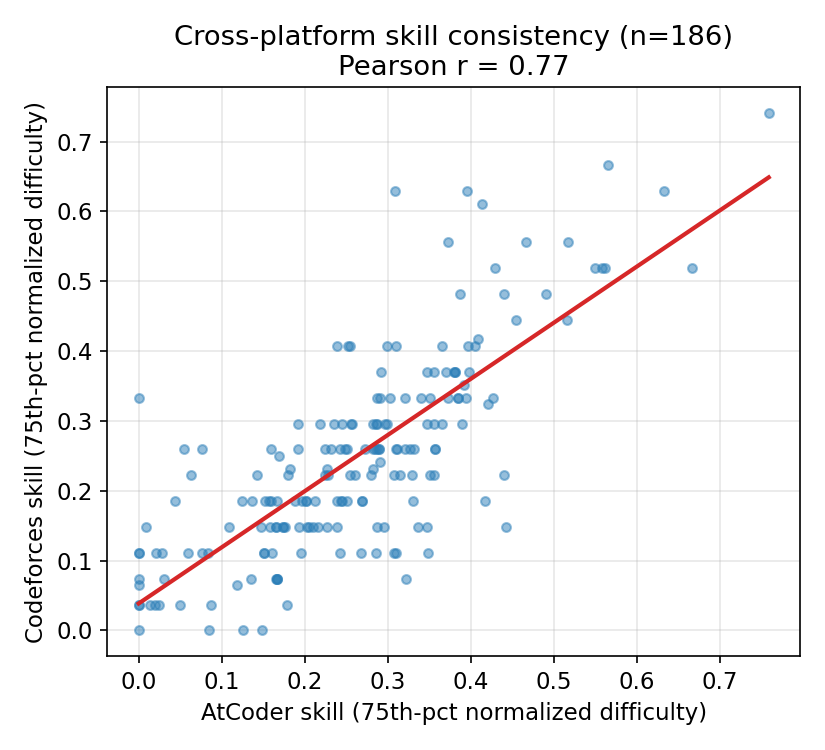
\includegraphics[width=\textwidth]{figures/xplat_skill_scatter.png}
\caption{Cross-platform skill consistency: CF vs.\ AtCoder skill, $r=0.77$.}
\label{fig:scatter}
\end{minipage}\hfill
\begin{minipage}{0.52\textwidth}\centering
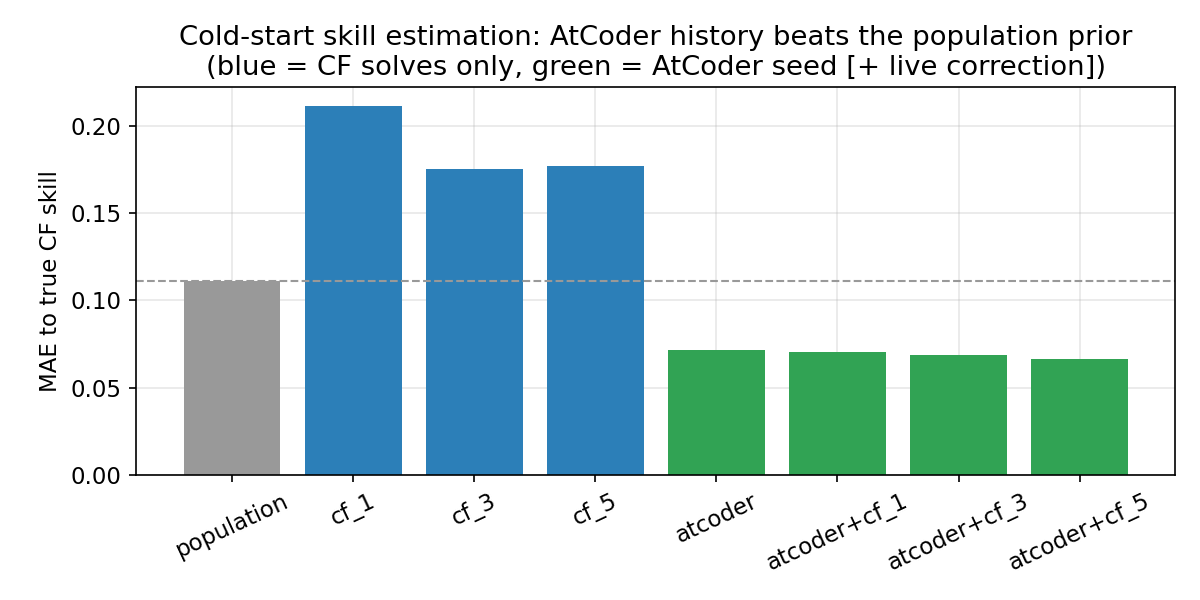
\includegraphics[width=\textwidth]{figures/coldstart_skill_mae.png}
\caption{Cold-start skill-estimation error. AtCoder history (green) beats the population
prior (dashed) and even several CF solves (blue).}
\label{fig:skillmae}
\end{minipage}
\end{figure}

Exploiting this, the online skill estimator (Section~\ref{sec:design-skill}) predicts a
brand-new Codeforces user's future skill from their AtCoder history alone.
Table~\ref{tab:adaptive} and Figure~\ref{fig:skillmae} quantify it over $184$ cohort
users: AtCoder-seeded estimation attains MAE $0.072$ against a population-prior MAE of
$0.111$ --- a \textbf{$35\%$ reduction} --- and a single CF solve is \emph{worse} than the
prior (MAE $0.211$) because one problem's difficulty is noisy, whereas AtCoder history is
abundant data. Seeding from AtCoder and then correcting with a few CF solves is best
($0.066$, $40\%$ better). Finally the estimate self-corrects online
(Figure~\ref{fig:convergence}): MAE falls monotonically from $0.108$ at one solve to
$0.081$ by twenty. This realises the ``unify on difficulty, assume solvability, correct
live'' design --- cross-platform history supplies a strong cold-start prior that native
evidence then refines --- and it is the positive resolution the premise required.

\begin{table}[h]
\centering
\caption{Cold-start CF-skill estimation error (MAE to a user's future 75th-percentile
solved difficulty; $n=184$). Green = uses AtCoder history.}
\label{tab:adaptive}
\small
\begin{tabular}{lcc}
\toprule
predictor & MAE & vs.\ population \\
\midrule
population prior            & 0.111 & --- \\
1 CF solve                  & 0.211 & $-90\%$ (worse) \\
3 CF solves                 & 0.175 & $-58\%$ (worse) \\
5 CF solves                 & 0.177 & $-59\%$ (worse) \\
AtCoder only (0 CF solves)  & \textbf{0.072} & $+35\%$ \\
AtCoder $+$ 5 CF (correct live) & \textbf{0.066} & $+40\%$ \\
\bottomrule
\end{tabular}
\end{table}

\begin{figure}[h]
\centering
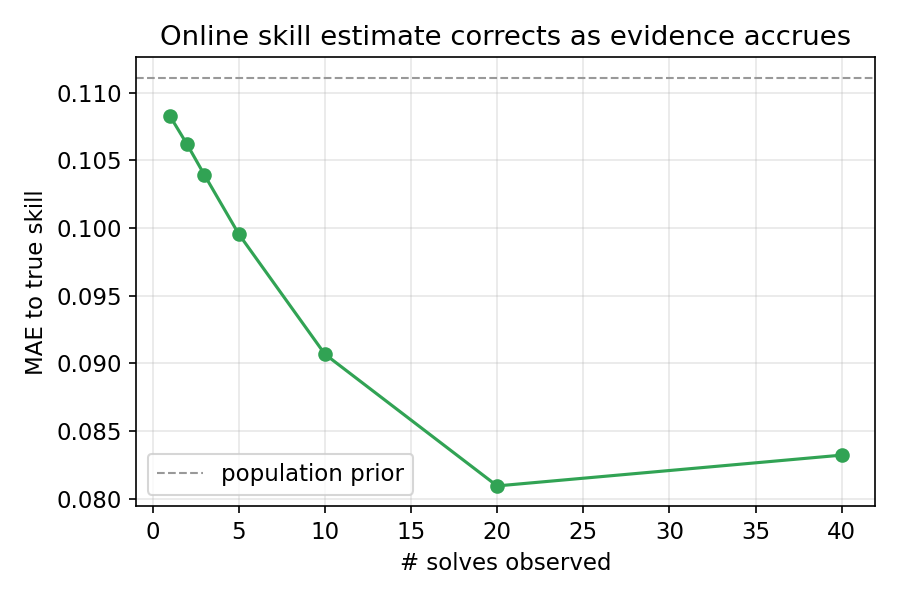
\includegraphics[width=0.56\textwidth]{figures/online_convergence.png}
\caption{The online skill estimate corrects as evidence accrues.}
\label{fig:convergence}
\end{figure}

%======================================================================
\section[Discussion \textnormal{\small(466 words)}]{Discussion}
\label{sec:discussion}
%======================================================================

\subsection{The Journey in Retrospect}
The project's arc is its argument. Both opening expectations were refuted, and each
refutation was diagnostic: the hybrid lost because the test population was not cold;
cross-platform collaboration lost because problem sets are disjoint and multi-platform
users uniformly experienced; and the win came from recognising that \emph{ability}, not
co-occurrence, is the transferable quantity.

\subsection{Interpretation against the Objectives}
Objectives O1--O3 (dataset, tagger, interaction data) and O7 (web app) are delivered as
described. O4 is answered by \RQ{1}: collaborative filtering is the right ranker,
decisively and significantly. O5 is answered by \RQ{2}: cold start is characterised
precisely, with a data-driven near-hard-switch policy replacing the assumed smooth ramp.
O6 --- the cross-platform question --- resolves into a dichotomy: \emph{collaborative}
transfer does not help (\RQ{3}), but \emph{skill} transfer does (\RQ{4}), validated at
$r=0.77$ and worth a $35$--$40\%$ cold-start improvement.

\subsection{Why the Negative Results are Informative}
Two counter-intuitive findings carry real weight. That content-based recommendation is
mis-aligned with next-solve prediction clarifies a common conflation: optimising for
pedagogical diversity is a different objective from predicting behaviour, and the two can
anti-correlate. That collaborative transfer fails across platforms bounds a widely assumed benefit and
confirms the cross-domain literature's warning: transfer needs shared items or a shared
latent cause. Skill is such a cause; co-occurrence over disjoint catalogues is not.

\subsection{Design Implications: When Each Signal Helps}
The results compose into a clear operating policy. Use CF to decide \emph{which} problem
for any user with $\geq1$ interaction. For a genuinely new user, fall back not to blind
popularity but to a cross-platform skill prior where available, recommending
difficulty-appropriate problems until native interactions accrue. Use the unified
difficulty scale, now validated, to calibrate challenge and to place users across
platforms. Treat content-based topic-gap recommendation as a \emph{diversification} tool,
not a next-solve predictor.

\subsection{Comparison to Prior Work}
Where prior programming-problem recommenders report a single metric on a single
platform~\cite{yera2018,zhao2018}, this work contributes a multi-model, multi-metric,
significance-tested comparison on a curated cross-platform dataset, and --- unlike systems
that assume cross-platform aggregation is beneficial --- measures it and finds the benefit
lies in ability transfer rather than collaborative transfer, consistent with cross-domain
theory~\cite{cantador2015,pan2010}.

\subsection{Threats to Validity}
\label{sec:threats}
\emph{Construct:} the cross-platform cohort is built by handle matching, which may
conflate distinct people or miss users with differing handles; AtCoder difficulty is a
community model estimate~\cite{kenkoooo2024}, not ground truth. \emph{Internal:} the
interaction data is solve-only (no failed attempts), so the skill model is evaluated on
solved-difficulty quantiles rather than success/failure calibration, and CF cannot use
negative signal. \emph{External:} the sample skews toward active, lower-rated learners and
toward Codeforces; results may differ for other populations or platforms.
\emph{Evaluation:} next-solve ranking rewards continuation and may understate the
pedagogical value of diversifying recommendations. None of these undermines the two
principal, significance-tested results, but each bounds their scope and motivates the
future work below.

%======================================================================
\section[Professional, Legal and Ethical Considerations \textnormal{\small(139 words)}]{Professional, Legal and Ethical Considerations}
\label{sec:ethics}
%======================================================================
Data was gathered only from public endpoints, with a polite fixed request delay,
exponential-backoff retries and resumable caching to minimise load, in keeping with the
platforms' terms and the kenkoooo project's request for considerate use. No private or
authenticated user data was collected beyond what public APIs expose. The web
application stores only what is necessary for accounts --- salted SHA-256 password hashes
and session tokens --- and the credential database is explicitly excluded from version
control. The handle-matching heuristic raises a mild re-identification consideration:
linking a Codeforces handle to an AtCoder handle by string equality is public
information but nonetheless joins two profiles; the cohort is used only in aggregate and
no individual is profiled or published. Course materials (exam papers, templates,
rubrics) are copyrighted and are likewise excluded from the repository. All third-party
libraries are open-source and cited.

%======================================================================
\section[Conclusion and Future Work \textnormal{\small(185 words)}]{Conclusion and Future Work}
\label{sec:conclusion}
%======================================================================
CPRS delivers a curated four-platform competitive-programming resource, an NLP tagger
that recovers missing topics on two of them, a working web application, and --- its analytical
core --- a rigorous, honest evaluation of recommendation across platforms. Collaborative
filtering is the strongest next-solve predictor; content-based ranking is mis-aligned
with the task; cold start is sharp and best met by a near-hard switch. The central
cross-platform question resolves into a clean dichotomy: collaborative transfer fails
across disjoint problem sets, but skill transfers strongly ($r=0.77$), and an online
cross-platform skill estimator converts this into a $35$--$40\%$ cold-start improvement.

Future work follows directly from the threats to validity. Incorporating failed attempts
would enable a full IRT/Elo solvability model and let CF exploit negative signal.
Extending the cohort with self-declared cross-platform identities would build a denser
bridge on which to revisit collaborative transfer. A sequence-aware model would test
whether interaction \emph{order} adds signal beyond the set of solves. Finally, and most
importantly, the difficulty-appropriate, online-correcting recommender should be evaluated
in a live user study measuring \emph{learning outcomes} rather than next-click prediction
--- the metric that ultimately matters for an educational tool.

%======================================================================
\appendix
\section{Full Metric Table}
\label{app:metrics}
Table~\ref{tab:full} reports all five metrics at $K\in\{5,10,20\}$ for the headline models.

\begin{table}[h]
\centering
\caption{Full metric table (selected models). H = HitRate, P = Precision, R = Recall, N =
\ndcg{}.}
\label{tab:full}
\scriptsize
\begin{tabular}{lcccccccccccc}
\toprule
 & H@5 & H@10 & H@20 & P@5 & P@10 & R@5 & R@10 & R@20 & N@5 & N@10 & N@20 & MRR@10 \\
\midrule
popularity  & 0.089 & 0.144 & 0.221 & 0.026 & 0.023 & 0.024 & 0.043 & 0.070 & 0.031 & 0.037 & 0.053 & 0.065 \\
diffmatch   & 0.024 & 0.041 & 0.069 & 0.006 & 0.004 & 0.003 & 0.005 & 0.009 & 0.005 & 0.006 & 0.007 & 0.020 \\
cf          & 0.216 & 0.295 & 0.386 & 0.081 & 0.059 & 0.079 & 0.118 & 0.169 & 0.086 & 0.096 & 0.125 & 0.130 \\
hybrid\_pop & 0.216 & 0.299 & 0.393 & 0.079 & 0.059 & 0.073 & 0.113 & 0.164 & 0.081 & 0.090 & 0.118 & 0.126 \\
\bottomrule
\end{tabular}
\end{table}

\section{Hyperparameters}
\label{app:hyper}
ALS: $64$ factors, regularisation $0.05$, $20$ iterations, confidence scale $\alpha=15$,
seed $42$. Content/diffmatch: difficulty Gaussian $\sigma=0.15$, stretch $0.10$ (content)
/ $0.05$ (diffmatch). Hybrid: $k_0=10$. Skill model: quantile $q=0.75$, learning rate
$\eta=0.02$. Tagger: TF--IDF $10\,000$ features, bigrams, sublinear TF; one-vs-rest
logistic regression; global threshold $0.5$; per-tag thresholds ranged $0.35$--$0.60$.
Split: leave-last-$N$, cap $10$ or $20\%$. Bootstrap: $2{,}000$ resamples.

\section{Unified Tag Taxonomy}
\label{app:taxonomy}
The 43 canonical topics: array, backtracking, bfs, binary\_search, bitmask, brute\_force,
combinatorics, constructive, data\_structures, design, dfs, divide\_and\_conquer,
dynamic\_programming, fft, game\_theory, geometry, graphs, greedy, hash\_table, hashing,
heap, implementation, linked\_list, math, matrix, monotonic\_stack, network\_flow,
number\_theory, prefix\_sum, probability, queue, recursion, segment\_tree, shortest\_paths,
simulation, sliding\_window, sorting, stack, string\_matching, strings, trees, trie,
two\_pointers.

\section{Reproduction}
\label{app:repro}
From committed raw data: \texttt{build\_interactions.py} $\to$ \texttt{split\_interactions.py}
$\to$ \texttt{evaluate.py} $\to$ \texttt{significance.py} $\to$ \texttt{coldstart\_sim.py};
cross-platform: \texttt{fetch\_crossplatform.py} $\to$ \texttt{build\_crossplatform.py}
$\to$ \texttt{eval\_crossplatform.py} $\to$ \texttt{eval\_adaptive.py}; CodeChef:
\texttt{enrich\_codechef.py} $\to$ \texttt{add\_codechef\_to\_dataset.py} $\to$
\texttt{auto\_tag\_codechef.py} (in that order --- the merge rewrites the CodeChef rows
the tagger then fills); figures: \texttt{make\_figures.py}. Seeds are fixed throughout.

%======================================================================
\begin{thebibliography}{99}
\small

\bibitem{wasik2018} S. Wasik, M. Antczak, J. Badura, A. Laskowski, and T. Sternal. 2018.
A Survey on Online Judge Systems and Their Applications. \emph{ACM Computing Surveys} 51,
1 (2018), 1--34.

\bibitem{behroozi2019} M. Behroozi, C. Parnin, and T. Barik. 2019. Hiring is Broken: What
Do Developers Say About Technical Interviews? In \emph{Proc.\ IEEE Symposium on Visual
Languages and Human-Centric Computing (VL/HCC)}. IEEE, 1--5.

\bibitem{boud2013} D. Boud and E. Molloy. 2013. Rethinking Models of Feedback for
Learning. \emph{Assessment \& Evaluation in Higher Education} 38, 6 (2013), 698--712.

\bibitem{ricci2015} F. Ricci, L. Rokach, and B. Shapira. 2015. \emph{Recommender Systems
Handbook} (2nd ed.). Springer.

\bibitem{lops2011} P. Lops, M. de Gemmis, and G. Semeraro. 2011. Content-based Recommender
Systems: State of the Art and Trends. In \emph{Recommender Systems Handbook}. Springer,
73--105.

\bibitem{burke2002} R. Burke. 2002. Hybrid Recommender Systems: Survey and Experiments.
\emph{User Modeling and User-Adapted Interaction} 12, 4 (2002), 331--370.

\bibitem{koren2009} Y. Koren, R. Bell, and C. Volinsky. 2009. Matrix Factorization
Techniques for Recommender Systems. \emph{Computer} 42, 8 (2009), 30--37.

\bibitem{hu2008} Y. Hu, Y. Koren, and C. Volinsky. 2008. Collaborative Filtering for
Implicit Feedback Datasets. In \emph{Proc.\ IEEE ICDM}. 263--272.

\bibitem{rendle2009} S. Rendle, C. Freudenthaler, Z. Gantner, and L. Schmidt-Thieme. 2009.
BPR: Bayesian Personalized Ranking from Implicit Feedback. In \emph{Proc.\ UAI}. 452--461.

\bibitem{schein2002} A. I. Schein, A. Popescul, L. H. Ungar, and D. M. Pennock. 2002.
Methods and Metrics for Cold-Start Recommendations. In \emph{Proc.\ ACM SIGIR}. 253--260.

\bibitem{cantador2015} I. Cantador, I. Fern\'andez-Tob\'ias, S. Berkovsky, and P. Cremonesi.
2015. Cross-Domain Recommender Systems. In \emph{Recommender Systems Handbook} (2nd ed.).
Springer, 919--959.

\bibitem{pan2010} W. Pan, E. W. Xiang, N. N. Liu, and Q. Yang. 2010. Transfer Learning in
Collaborative Filtering for Sparsity Reduction. In \emph{Proc.\ AAAI}. 230--235.

\bibitem{hidasi2016} B. Hidasi, A. Karatzoglou, L. Baltrunas, and D. Tikk. 2016.
Session-based Recommendations with Recurrent Neural Networks. In \emph{Proc.\ ICLR}.

\bibitem{corbett1994} A. T. Corbett and J. R. Anderson. 1994. Knowledge Tracing: Modeling
the Acquisition of Procedural Knowledge. \emph{User Modeling and User-Adapted Interaction}
4, 4 (1994), 253--278.

\bibitem{piech2015} C. Piech, et al. 2015. Deep Knowledge Tracing. In \emph{Advances in
Neural Information Processing Systems (NeurIPS)}. 505--513.

\bibitem{pelanek2017} R. Pel\'anek. 2017. Bayesian Knowledge Tracing, Logistic Models, and
Beyond: An Overview of Learner Modeling Techniques. \emph{User Modeling and User-Adapted
Interaction} 27, 3--5 (2017), 313--350.

\bibitem{elo1978} A. E. Elo. 1978. \emph{The Rating of Chessplayers, Past and Present}.
Arco Publishing.

\bibitem{vygotsky1978} L. S. Vygotsky. 1978. \emph{Mind in Society: The Development of
Higher Psychological Processes}. Harvard University Press.

\bibitem{yera2018} R. Yera Toledo, Y. Caballero Mota, and L. Mart\'{\i}nez. 2018. A
Recommender System for Programming Online Judges Using Fuzzy Information Modeling.
\emph{Informatics} 5, 2 (2018), Article 17.

\bibitem{zhao2018} W. X. Zhao, W. Zhang, Y. He, X. Xie, and J.-R. Wen. 2018.
Automatically Learning Topics and Difficulty Levels of Problems in Online Judge Systems.
\emph{ACM Transactions on Information Systems} 36, 3 (2018), Article 27, 33 pages.

\bibitem{jarvelin2002} K. J\"arvelin and J. Kek\"al\"ainen. 2002. Cumulated Gain-based
Evaluation of IR Techniques. \emph{ACM Transactions on Information Systems} 20, 4 (2002),
422--446.

\bibitem{cremonesi2010} P. Cremonesi, Y. Koren, and R. Turrin. 2010. Performance of
Recommender Algorithms on Top-N Recommendation Tasks. In \emph{Proc.\ ACM RecSys}. 39--46.

\bibitem{dacrema2019} M. F. Dacrema, P. Cremonesi, and D. Jannach. 2019. Are We Really
Making Much Progress? A Worrying Analysis of Recent Neural Recommendation Approaches. In
\emph{Proc.\ ACM RecSys}. 101--109.

\bibitem{wilcoxon1945} F. Wilcoxon. 1945. Individual Comparisons by Ranking Methods.
\emph{Biometrics Bulletin} 1, 6 (1945), 80--83.

\bibitem{kenkoooo2024} kenkoooo. 2024. AtCoder Problems: API and Difficulty Models.
\url{https://kenkoooo.com/atcoder}. Accessed 2026.

\end{thebibliography}

\end{document}
